% Start preamble
\documentclass[12pt,a4paper]{article}
\usepackage{geometry}
 \geometry{
 a4paper,
 total={170mm,257mm},
 left=20mm,
 top=20mm,
 }
\usepackage[utf8]{inputenc}
\usepackage[T1]{fontenc}
\usepackage[pdftex]{graphicx}
\graphicspath{{./}}
\usepackage{enumitem}
\usepackage{pdfpages}
\usepackage{hyperref}
\usepackage{tikz}
\usepackage{attachfile}
\usepackage{epstopdf}
\usepackage{array}
%\usepackage[table]{xcolor,colorbl}
\setlength{\textwidth}{16cm}
\setlength{\oddsidemargin}{-0.5cm}
\setlength{\evensidemargin}{-0.5cm}
%\setlenght{\headsep}{0cm}
\setlength\parindent{0pt}
%\setlength{\extrarowheight}{3pt}
\usepackage{listings}
%\usepackage{xcolor}

 %%%%%%%%%%%%%%%%%%%%%%%%%%%%%%%%%%%%%%%%%%%%%%%%%%%%%%%%%%%%%%%%%%%%%%%%%%%%%%%% 
%%% ~ Arduino Language - Arduino IDE Colors ~                                  %%%
%%%                                                                            %%%
%%% Kyle Rocha-Brownell | 10/2/2017 | No Licence                               %%%
%%% -------------------------------------------------------------------------- %%%
%%%                                                                            %%%
%%% Place this file in your working directory (next to the latex file you're   %%%
%%% working on).  To add it to your project, place:                            %%%
%%%     %%%%%%%%%%%%%%%%%%%%%%%%%%%%%%%%%%%%%%%%%%%%%%%%%%%%%%%%%%%%%%%%%%%%%%%%%%%%%%%% 
%%% ~ Arduino Language - Arduino IDE Colors ~                                  %%%
%%%                                                                            %%%
%%% Kyle Rocha-Brownell | 10/2/2017 | No Licence                               %%%
%%% -------------------------------------------------------------------------- %%%
%%%                                                                            %%%
%%% Place this file in your working directory (next to the latex file you're   %%%
%%% working on).  To add it to your project, place:                            %%%
%%%     %%%%%%%%%%%%%%%%%%%%%%%%%%%%%%%%%%%%%%%%%%%%%%%%%%%%%%%%%%%%%%%%%%%%%%%%%%%%%%%% 
%%% ~ Arduino Language - Arduino IDE Colors ~                                  %%%
%%%                                                                            %%%
%%% Kyle Rocha-Brownell | 10/2/2017 | No Licence                               %%%
%%% -------------------------------------------------------------------------- %%%
%%%                                                                            %%%
%%% Place this file in your working directory (next to the latex file you're   %%%
%%% working on).  To add it to your project, place:                            %%%
%%%    \input{arduinoLanguage.tex}                                             %%%
%%% somewhere before \begin{document} in your latex file.                      %%%
%%%                                                                            %%%
%%% In your document, place your arduino code between:                         %%%
%%%   \begin{lstlisting}[language=Arduino]                                     %%%
%%% and:                                                                       %%%
%%%   \end{lstlisting}                                                         %%%
%%%                                                                            %%%
%%% Or create your own style to add non-built-in functions and variables.      %%%
%%%                                                                            %%%
 %%%%%%%%%%%%%%%%%%%%%%%%%%%%%%%%%%%%%%%%%%%%%%%%%%%%%%%%%%%%%%%%%%%%%%%%%%%%%%%% 

\usepackage{color}
\usepackage{listings}    
\usepackage{courier}

%%% Define Custom IDE Colors %%%
\definecolor{arduinoGreen}    {rgb} {0.17, 0.43, 0.01}
\definecolor{arduinoGrey}     {rgb} {0.47, 0.47, 0.33}
\definecolor{arduinoOrange}   {rgb} {0.8 , 0.4 , 0   }
\definecolor{arduinoBlue}     {rgb} {0.01, 0.61, 0.98}
\definecolor{arduinoDarkBlue} {rgb} {0.0 , 0.2 , 0.5 }

%%% Define Arduino Language %%%
\lstdefinelanguage{Arduino}{
  language=C++, % begin with default C++ settings 
%
%
  %%% Keyword Color Group 1 %%%  (called KEYWORD3 by arduino)
  keywordstyle=\color{arduinoGreen},   
  deletekeywords={  % remove all arduino keywords that might be in c++
                break, case, override, final, continue, default, do, else, for, 
                if, return, goto, switch, throw, try, while, setup, loop, export, 
                not, or, and, xor, include, define, elif, else, error, if, ifdef, 
                ifndef, pragma, warning,
                HIGH, LOW, INPUT, INPUT_PULLUP, OUTPUT, DEC, BIN, HEX, OCT, PI, 
                HALF_PI, TWO_PI, LSBFIRST, MSBFIRST, CHANGE, FALLING, RISING, 
                DEFAULT, EXTERNAL, INTERNAL, INTERNAL1V1, INTERNAL2V56, LED_BUILTIN, 
                LED_BUILTIN_RX, LED_BUILTIN_TX, DIGITAL_MESSAGE, FIRMATA_STRING, 
                ANALOG_MESSAGE, REPORT_DIGITAL, REPORT_ANALOG, SET_PIN_MODE, 
                SYSTEM_RESET, SYSEX_START, auto, int8_t, int16_t, int32_t, int64_t, 
                uint8_t, uint16_t, uint32_t, uint64_t, char16_t, char32_t, operator, 
                enum, delete, bool, boolean, byte, char, const, false, float, double, 
                null, NULL, int, long, new, private, protected, public, short, 
                signed, static, volatile, String, void, true, unsigned, word, array, 
                sizeof, dynamic_cast, typedef, const_cast, struct, static_cast, union, 
                friend, extern, class, reinterpret_cast, register, explicit, inline, 
                _Bool, complex, _Complex, _Imaginary, atomic_bool, atomic_char, 
                atomic_schar, atomic_uchar, atomic_short, atomic_ushort, atomic_int, 
                atomic_uint, atomic_long, atomic_ulong, atomic_llong, atomic_ullong, 
                virtual, PROGMEM,
                Serial, Serial1, Serial2, Serial3, SerialUSB, Keyboard, Mouse,
                abs, acos, asin, atan, atan2, ceil, constrain, cos, degrees, exp, 
                floor, log, map, max, min, radians, random, randomSeed, round, sin, 
                sq, sqrt, tan, pow, bitRead, bitWrite, bitSet, bitClear, bit, 
                highByte, lowByte, analogReference, analogRead, 
                analogReadResolution, analogWrite, analogWriteResolution, 
                attachInterrupt, detachInterrupt, digitalPinToInterrupt, delay, 
                delayMicroseconds, digitalWrite, digitalRead, interrupts, millis, 
                micros, noInterrupts, noTone, pinMode, pulseIn, pulseInLong, shiftIn, 
                shiftOut, tone, yield, Stream, begin, end, peek, read, print, 
                println, available, availableForWrite, flush, setTimeout, find, 
                findUntil, parseInt, parseFloat, readBytes, readBytesUntil, readString, 
                readStringUntil, trim, toUpperCase, toLowerCase, charAt, compareTo, 
                concat, endsWith, startsWith, equals, equalsIgnoreCase, getBytes, 
                indexOf, lastIndexOf, length, replace, setCharAt, substring, 
                toCharArray, toInt, press, release, releaseAll, accept, click, move, 
                isPressed, isAlphaNumeric, isAlpha, isAscii, isWhitespace, isControl, 
                isDigit, isGraph, isLowerCase, isPrintable, isPunct, isSpace, 
                isUpperCase, isHexadecimalDigit, 
                }, 
  morekeywords={   % add arduino structures to group 1
                break, case, override, final, continue, default, do, else, for, 
                if, return, goto, switch, throw, try, while, setup, loop, export, 
                not, or, and, xor, include, define, elif, else, error, if, ifdef, 
                ifndef, pragma, warning,
                }, 
% 
%
  %%% Keyword Color Group 2 %%%  (called LITERAL1 by arduino)
  keywordstyle=[2]\color{arduinoBlue},   
  keywords=[2]{   % add variables and dataTypes as 2nd group  
                HIGH, LOW, INPUT, INPUT_PULLUP, OUTPUT, DEC, BIN, HEX, OCT, PI, 
                HALF_PI, TWO_PI, LSBFIRST, MSBFIRST, CHANGE, FALLING, RISING, 
                DEFAULT, EXTERNAL, INTERNAL, INTERNAL1V1, INTERNAL2V56, LED_BUILTIN, 
                LED_BUILTIN_RX, LED_BUILTIN_TX, DIGITAL_MESSAGE, FIRMATA_STRING, 
                ANALOG_MESSAGE, REPORT_DIGITAL, REPORT_ANALOG, SET_PIN_MODE, 
                SYSTEM_RESET, SYSEX_START, auto, int8_t, int16_t, int32_t, int64_t, 
                uint8_t, uint16_t, uint32_t, uint64_t, char16_t, char32_t, operator, 
                enum, delete, bool, boolean, byte, char, const, false, float, double, 
                null, NULL, int, long, new, private, protected, public, short, 
                signed, static, volatile, String, void, true, unsigned, word, array, 
                sizeof, dynamic_cast, typedef, const_cast, struct, static_cast, union, 
                friend, extern, class, reinterpret_cast, register, explicit, inline, 
                _Bool, complex, _Complex, _Imaginary, atomic_bool, atomic_char, 
                atomic_schar, atomic_uchar, atomic_short, atomic_ushort, atomic_int, 
                atomic_uint, atomic_long, atomic_ulong, atomic_llong, atomic_ullong, 
                virtual, PROGMEM,
                },  
% 
%
  %%% Keyword Color Group 3 %%%  (called KEYWORD1 by arduino)
  keywordstyle=[3]\bfseries\color{arduinoOrange},
  keywords=[3]{  % add built-in functions as a 3rd group
                Serial, Serial1, Serial2, Serial3, SerialUSB, Keyboard, Mouse,
                },      
%
%
  %%% Keyword Color Group 4 %%%  (called KEYWORD2 by arduino)
  keywordstyle=[4]\color{arduinoOrange},
  keywords=[4]{  % add more built-in functions as a 4th group
                abs, acos, asin, atan, atan2, ceil, constrain, cos, degrees, exp, 
                floor, log, map, max, min, radians, random, randomSeed, round, sin, 
                sq, sqrt, tan, pow, bitRead, bitWrite, bitSet, bitClear, bit, 
                highByte, lowByte, analogReference, analogRead, 
                analogReadResolution, analogWrite, analogWriteResolution, 
                attachInterrupt, detachInterrupt, digitalPinToInterrupt, delay, 
                delayMicroseconds, digitalWrite, digitalRead, interrupts, millis, 
                micros, noInterrupts, noTone, pinMode, pulseIn, pulseInLong, shiftIn, 
                shiftOut, tone, yield, Stream, begin, end, peek, read, print, 
                println, available, availableForWrite, flush, setTimeout, find, 
                findUntil, parseInt, parseFloat, readBytes, readBytesUntil, readString, 
                readStringUntil, trim, toUpperCase, toLowerCase, charAt, compareTo, 
                concat, endsWith, startsWith, equals, equalsIgnoreCase, getBytes, 
                indexOf, lastIndexOf, length, replace, setCharAt, substring, 
                toCharArray, toInt, press, release, releaseAll, accept, click, move, 
                isPressed, isAlphaNumeric, isAlpha, isAscii, isWhitespace, isControl, 
                isDigit, isGraph, isLowerCase, isPrintable, isPunct, isSpace, 
                isUpperCase, isHexadecimalDigit, 
                },      
%
%
  %%% Set Other Colors %%%
  stringstyle=\color{arduinoDarkBlue},    
  commentstyle=\color{arduinoGrey},    
%          
%   
  %%%% Line Numbering %%%%
%  numbers=left,                    
%  numbersep=5pt,                   
%  numberstyle=\color{arduinoGrey},    
  %stepnumber=2,                      % show every 2 line numbers
%
%
  %%%% Code Box Style %%%%
  breaklines=true,                    % wordwrapping
  tabsize=8,         
  basicstyle=\ttfamily  
}
                                             %%%
%%% somewhere before \begin{document} in your latex file.                      %%%
%%%                                                                            %%%
%%% In your document, place your arduino code between:                         %%%
%%%   \begin{lstlisting}[language=Arduino]                                     %%%
%%% and:                                                                       %%%
%%%   \end{lstlisting}                                                         %%%
%%%                                                                            %%%
%%% Or create your own style to add non-built-in functions and variables.      %%%
%%%                                                                            %%%
 %%%%%%%%%%%%%%%%%%%%%%%%%%%%%%%%%%%%%%%%%%%%%%%%%%%%%%%%%%%%%%%%%%%%%%%%%%%%%%%% 

\usepackage{color}
\usepackage{listings}    
\usepackage{courier}

%%% Define Custom IDE Colors %%%
\definecolor{arduinoGreen}    {rgb} {0.17, 0.43, 0.01}
\definecolor{arduinoGrey}     {rgb} {0.47, 0.47, 0.33}
\definecolor{arduinoOrange}   {rgb} {0.8 , 0.4 , 0   }
\definecolor{arduinoBlue}     {rgb} {0.01, 0.61, 0.98}
\definecolor{arduinoDarkBlue} {rgb} {0.0 , 0.2 , 0.5 }

%%% Define Arduino Language %%%
\lstdefinelanguage{Arduino}{
  language=C++, % begin with default C++ settings 
%
%
  %%% Keyword Color Group 1 %%%  (called KEYWORD3 by arduino)
  keywordstyle=\color{arduinoGreen},   
  deletekeywords={  % remove all arduino keywords that might be in c++
                break, case, override, final, continue, default, do, else, for, 
                if, return, goto, switch, throw, try, while, setup, loop, export, 
                not, or, and, xor, include, define, elif, else, error, if, ifdef, 
                ifndef, pragma, warning,
                HIGH, LOW, INPUT, INPUT_PULLUP, OUTPUT, DEC, BIN, HEX, OCT, PI, 
                HALF_PI, TWO_PI, LSBFIRST, MSBFIRST, CHANGE, FALLING, RISING, 
                DEFAULT, EXTERNAL, INTERNAL, INTERNAL1V1, INTERNAL2V56, LED_BUILTIN, 
                LED_BUILTIN_RX, LED_BUILTIN_TX, DIGITAL_MESSAGE, FIRMATA_STRING, 
                ANALOG_MESSAGE, REPORT_DIGITAL, REPORT_ANALOG, SET_PIN_MODE, 
                SYSTEM_RESET, SYSEX_START, auto, int8_t, int16_t, int32_t, int64_t, 
                uint8_t, uint16_t, uint32_t, uint64_t, char16_t, char32_t, operator, 
                enum, delete, bool, boolean, byte, char, const, false, float, double, 
                null, NULL, int, long, new, private, protected, public, short, 
                signed, static, volatile, String, void, true, unsigned, word, array, 
                sizeof, dynamic_cast, typedef, const_cast, struct, static_cast, union, 
                friend, extern, class, reinterpret_cast, register, explicit, inline, 
                _Bool, complex, _Complex, _Imaginary, atomic_bool, atomic_char, 
                atomic_schar, atomic_uchar, atomic_short, atomic_ushort, atomic_int, 
                atomic_uint, atomic_long, atomic_ulong, atomic_llong, atomic_ullong, 
                virtual, PROGMEM,
                Serial, Serial1, Serial2, Serial3, SerialUSB, Keyboard, Mouse,
                abs, acos, asin, atan, atan2, ceil, constrain, cos, degrees, exp, 
                floor, log, map, max, min, radians, random, randomSeed, round, sin, 
                sq, sqrt, tan, pow, bitRead, bitWrite, bitSet, bitClear, bit, 
                highByte, lowByte, analogReference, analogRead, 
                analogReadResolution, analogWrite, analogWriteResolution, 
                attachInterrupt, detachInterrupt, digitalPinToInterrupt, delay, 
                delayMicroseconds, digitalWrite, digitalRead, interrupts, millis, 
                micros, noInterrupts, noTone, pinMode, pulseIn, pulseInLong, shiftIn, 
                shiftOut, tone, yield, Stream, begin, end, peek, read, print, 
                println, available, availableForWrite, flush, setTimeout, find, 
                findUntil, parseInt, parseFloat, readBytes, readBytesUntil, readString, 
                readStringUntil, trim, toUpperCase, toLowerCase, charAt, compareTo, 
                concat, endsWith, startsWith, equals, equalsIgnoreCase, getBytes, 
                indexOf, lastIndexOf, length, replace, setCharAt, substring, 
                toCharArray, toInt, press, release, releaseAll, accept, click, move, 
                isPressed, isAlphaNumeric, isAlpha, isAscii, isWhitespace, isControl, 
                isDigit, isGraph, isLowerCase, isPrintable, isPunct, isSpace, 
                isUpperCase, isHexadecimalDigit, 
                }, 
  morekeywords={   % add arduino structures to group 1
                break, case, override, final, continue, default, do, else, for, 
                if, return, goto, switch, throw, try, while, setup, loop, export, 
                not, or, and, xor, include, define, elif, else, error, if, ifdef, 
                ifndef, pragma, warning,
                }, 
% 
%
  %%% Keyword Color Group 2 %%%  (called LITERAL1 by arduino)
  keywordstyle=[2]\color{arduinoBlue},   
  keywords=[2]{   % add variables and dataTypes as 2nd group  
                HIGH, LOW, INPUT, INPUT_PULLUP, OUTPUT, DEC, BIN, HEX, OCT, PI, 
                HALF_PI, TWO_PI, LSBFIRST, MSBFIRST, CHANGE, FALLING, RISING, 
                DEFAULT, EXTERNAL, INTERNAL, INTERNAL1V1, INTERNAL2V56, LED_BUILTIN, 
                LED_BUILTIN_RX, LED_BUILTIN_TX, DIGITAL_MESSAGE, FIRMATA_STRING, 
                ANALOG_MESSAGE, REPORT_DIGITAL, REPORT_ANALOG, SET_PIN_MODE, 
                SYSTEM_RESET, SYSEX_START, auto, int8_t, int16_t, int32_t, int64_t, 
                uint8_t, uint16_t, uint32_t, uint64_t, char16_t, char32_t, operator, 
                enum, delete, bool, boolean, byte, char, const, false, float, double, 
                null, NULL, int, long, new, private, protected, public, short, 
                signed, static, volatile, String, void, true, unsigned, word, array, 
                sizeof, dynamic_cast, typedef, const_cast, struct, static_cast, union, 
                friend, extern, class, reinterpret_cast, register, explicit, inline, 
                _Bool, complex, _Complex, _Imaginary, atomic_bool, atomic_char, 
                atomic_schar, atomic_uchar, atomic_short, atomic_ushort, atomic_int, 
                atomic_uint, atomic_long, atomic_ulong, atomic_llong, atomic_ullong, 
                virtual, PROGMEM,
                },  
% 
%
  %%% Keyword Color Group 3 %%%  (called KEYWORD1 by arduino)
  keywordstyle=[3]\bfseries\color{arduinoOrange},
  keywords=[3]{  % add built-in functions as a 3rd group
                Serial, Serial1, Serial2, Serial3, SerialUSB, Keyboard, Mouse,
                },      
%
%
  %%% Keyword Color Group 4 %%%  (called KEYWORD2 by arduino)
  keywordstyle=[4]\color{arduinoOrange},
  keywords=[4]{  % add more built-in functions as a 4th group
                abs, acos, asin, atan, atan2, ceil, constrain, cos, degrees, exp, 
                floor, log, map, max, min, radians, random, randomSeed, round, sin, 
                sq, sqrt, tan, pow, bitRead, bitWrite, bitSet, bitClear, bit, 
                highByte, lowByte, analogReference, analogRead, 
                analogReadResolution, analogWrite, analogWriteResolution, 
                attachInterrupt, detachInterrupt, digitalPinToInterrupt, delay, 
                delayMicroseconds, digitalWrite, digitalRead, interrupts, millis, 
                micros, noInterrupts, noTone, pinMode, pulseIn, pulseInLong, shiftIn, 
                shiftOut, tone, yield, Stream, begin, end, peek, read, print, 
                println, available, availableForWrite, flush, setTimeout, find, 
                findUntil, parseInt, parseFloat, readBytes, readBytesUntil, readString, 
                readStringUntil, trim, toUpperCase, toLowerCase, charAt, compareTo, 
                concat, endsWith, startsWith, equals, equalsIgnoreCase, getBytes, 
                indexOf, lastIndexOf, length, replace, setCharAt, substring, 
                toCharArray, toInt, press, release, releaseAll, accept, click, move, 
                isPressed, isAlphaNumeric, isAlpha, isAscii, isWhitespace, isControl, 
                isDigit, isGraph, isLowerCase, isPrintable, isPunct, isSpace, 
                isUpperCase, isHexadecimalDigit, 
                },      
%
%
  %%% Set Other Colors %%%
  stringstyle=\color{arduinoDarkBlue},    
  commentstyle=\color{arduinoGrey},    
%          
%   
  %%%% Line Numbering %%%%
%  numbers=left,                    
%  numbersep=5pt,                   
%  numberstyle=\color{arduinoGrey},    
  %stepnumber=2,                      % show every 2 line numbers
%
%
  %%%% Code Box Style %%%%
  breaklines=true,                    % wordwrapping
  tabsize=8,         
  basicstyle=\ttfamily  
}
                                             %%%
%%% somewhere before \begin{document} in your latex file.                      %%%
%%%                                                                            %%%
%%% In your document, place your arduino code between:                         %%%
%%%   \begin{lstlisting}[language=Arduino]                                     %%%
%%% and:                                                                       %%%
%%%   \end{lstlisting}                                                         %%%
%%%                                                                            %%%
%%% Or create your own style to add non-built-in functions and variables.      %%%
%%%                                                                            %%%
 %%%%%%%%%%%%%%%%%%%%%%%%%%%%%%%%%%%%%%%%%%%%%%%%%%%%%%%%%%%%%%%%%%%%%%%%%%%%%%%% 

\usepackage{color}
\usepackage{listings}    
\usepackage{courier}

%%% Define Custom IDE Colors %%%
\definecolor{arduinoGreen}    {rgb} {0.17, 0.43, 0.01}
\definecolor{arduinoGrey}     {rgb} {0.47, 0.47, 0.33}
\definecolor{arduinoOrange}   {rgb} {0.8 , 0.4 , 0   }
\definecolor{arduinoBlue}     {rgb} {0.01, 0.61, 0.98}
\definecolor{arduinoDarkBlue} {rgb} {0.0 , 0.2 , 0.5 }

%%% Define Arduino Language %%%
\lstdefinelanguage{Arduino}{
  language=C++, % begin with default C++ settings 
%
%
  %%% Keyword Color Group 1 %%%  (called KEYWORD3 by arduino)
  keywordstyle=\color{arduinoGreen},   
  deletekeywords={  % remove all arduino keywords that might be in c++
                break, case, override, final, continue, default, do, else, for, 
                if, return, goto, switch, throw, try, while, setup, loop, export, 
                not, or, and, xor, include, define, elif, else, error, if, ifdef, 
                ifndef, pragma, warning,
                HIGH, LOW, INPUT, INPUT_PULLUP, OUTPUT, DEC, BIN, HEX, OCT, PI, 
                HALF_PI, TWO_PI, LSBFIRST, MSBFIRST, CHANGE, FALLING, RISING, 
                DEFAULT, EXTERNAL, INTERNAL, INTERNAL1V1, INTERNAL2V56, LED_BUILTIN, 
                LED_BUILTIN_RX, LED_BUILTIN_TX, DIGITAL_MESSAGE, FIRMATA_STRING, 
                ANALOG_MESSAGE, REPORT_DIGITAL, REPORT_ANALOG, SET_PIN_MODE, 
                SYSTEM_RESET, SYSEX_START, auto, int8_t, int16_t, int32_t, int64_t, 
                uint8_t, uint16_t, uint32_t, uint64_t, char16_t, char32_t, operator, 
                enum, delete, bool, boolean, byte, char, const, false, float, double, 
                null, NULL, int, long, new, private, protected, public, short, 
                signed, static, volatile, String, void, true, unsigned, word, array, 
                sizeof, dynamic_cast, typedef, const_cast, struct, static_cast, union, 
                friend, extern, class, reinterpret_cast, register, explicit, inline, 
                _Bool, complex, _Complex, _Imaginary, atomic_bool, atomic_char, 
                atomic_schar, atomic_uchar, atomic_short, atomic_ushort, atomic_int, 
                atomic_uint, atomic_long, atomic_ulong, atomic_llong, atomic_ullong, 
                virtual, PROGMEM,
                Serial, Serial1, Serial2, Serial3, SerialUSB, Keyboard, Mouse,
                abs, acos, asin, atan, atan2, ceil, constrain, cos, degrees, exp, 
                floor, log, map, max, min, radians, random, randomSeed, round, sin, 
                sq, sqrt, tan, pow, bitRead, bitWrite, bitSet, bitClear, bit, 
                highByte, lowByte, analogReference, analogRead, 
                analogReadResolution, analogWrite, analogWriteResolution, 
                attachInterrupt, detachInterrupt, digitalPinToInterrupt, delay, 
                delayMicroseconds, digitalWrite, digitalRead, interrupts, millis, 
                micros, noInterrupts, noTone, pinMode, pulseIn, pulseInLong, shiftIn, 
                shiftOut, tone, yield, Stream, begin, end, peek, read, print, 
                println, available, availableForWrite, flush, setTimeout, find, 
                findUntil, parseInt, parseFloat, readBytes, readBytesUntil, readString, 
                readStringUntil, trim, toUpperCase, toLowerCase, charAt, compareTo, 
                concat, endsWith, startsWith, equals, equalsIgnoreCase, getBytes, 
                indexOf, lastIndexOf, length, replace, setCharAt, substring, 
                toCharArray, toInt, press, release, releaseAll, accept, click, move, 
                isPressed, isAlphaNumeric, isAlpha, isAscii, isWhitespace, isControl, 
                isDigit, isGraph, isLowerCase, isPrintable, isPunct, isSpace, 
                isUpperCase, isHexadecimalDigit, 
                }, 
  morekeywords={   % add arduino structures to group 1
                break, case, override, final, continue, default, do, else, for, 
                if, return, goto, switch, throw, try, while, setup, loop, export, 
                not, or, and, xor, include, define, elif, else, error, if, ifdef, 
                ifndef, pragma, warning,
                }, 
% 
%
  %%% Keyword Color Group 2 %%%  (called LITERAL1 by arduino)
  keywordstyle=[2]\color{arduinoBlue},   
  keywords=[2]{   % add variables and dataTypes as 2nd group  
                HIGH, LOW, INPUT, INPUT_PULLUP, OUTPUT, DEC, BIN, HEX, OCT, PI, 
                HALF_PI, TWO_PI, LSBFIRST, MSBFIRST, CHANGE, FALLING, RISING, 
                DEFAULT, EXTERNAL, INTERNAL, INTERNAL1V1, INTERNAL2V56, LED_BUILTIN, 
                LED_BUILTIN_RX, LED_BUILTIN_TX, DIGITAL_MESSAGE, FIRMATA_STRING, 
                ANALOG_MESSAGE, REPORT_DIGITAL, REPORT_ANALOG, SET_PIN_MODE, 
                SYSTEM_RESET, SYSEX_START, auto, int8_t, int16_t, int32_t, int64_t, 
                uint8_t, uint16_t, uint32_t, uint64_t, char16_t, char32_t, operator, 
                enum, delete, bool, boolean, byte, char, const, false, float, double, 
                null, NULL, int, long, new, private, protected, public, short, 
                signed, static, volatile, String, void, true, unsigned, word, array, 
                sizeof, dynamic_cast, typedef, const_cast, struct, static_cast, union, 
                friend, extern, class, reinterpret_cast, register, explicit, inline, 
                _Bool, complex, _Complex, _Imaginary, atomic_bool, atomic_char, 
                atomic_schar, atomic_uchar, atomic_short, atomic_ushort, atomic_int, 
                atomic_uint, atomic_long, atomic_ulong, atomic_llong, atomic_ullong, 
                virtual, PROGMEM,
                },  
% 
%
  %%% Keyword Color Group 3 %%%  (called KEYWORD1 by arduino)
  keywordstyle=[3]\bfseries\color{arduinoOrange},
  keywords=[3]{  % add built-in functions as a 3rd group
                Serial, Serial1, Serial2, Serial3, SerialUSB, Keyboard, Mouse,
                },      
%
%
  %%% Keyword Color Group 4 %%%  (called KEYWORD2 by arduino)
  keywordstyle=[4]\color{arduinoOrange},
  keywords=[4]{  % add more built-in functions as a 4th group
                abs, acos, asin, atan, atan2, ceil, constrain, cos, degrees, exp, 
                floor, log, map, max, min, radians, random, randomSeed, round, sin, 
                sq, sqrt, tan, pow, bitRead, bitWrite, bitSet, bitClear, bit, 
                highByte, lowByte, analogReference, analogRead, 
                analogReadResolution, analogWrite, analogWriteResolution, 
                attachInterrupt, detachInterrupt, digitalPinToInterrupt, delay, 
                delayMicroseconds, digitalWrite, digitalRead, interrupts, millis, 
                micros, noInterrupts, noTone, pinMode, pulseIn, pulseInLong, shiftIn, 
                shiftOut, tone, yield, Stream, begin, end, peek, read, print, 
                println, available, availableForWrite, flush, setTimeout, find, 
                findUntil, parseInt, parseFloat, readBytes, readBytesUntil, readString, 
                readStringUntil, trim, toUpperCase, toLowerCase, charAt, compareTo, 
                concat, endsWith, startsWith, equals, equalsIgnoreCase, getBytes, 
                indexOf, lastIndexOf, length, replace, setCharAt, substring, 
                toCharArray, toInt, press, release, releaseAll, accept, click, move, 
                isPressed, isAlphaNumeric, isAlpha, isAscii, isWhitespace, isControl, 
                isDigit, isGraph, isLowerCase, isPrintable, isPunct, isSpace, 
                isUpperCase, isHexadecimalDigit, 
                },      
%
%
  %%% Set Other Colors %%%
  stringstyle=\color{arduinoDarkBlue},    
  commentstyle=\color{arduinoGrey},    
%          
%   
  %%%% Line Numbering %%%%
%  numbers=left,                    
%  numbersep=5pt,                   
%  numberstyle=\color{arduinoGrey},    
  %stepnumber=2,                      % show every 2 line numbers
%
%
  %%%% Code Box Style %%%%
  breaklines=true,                    % wordwrapping
  tabsize=8,         
  basicstyle=\ttfamily  
}

%%%%%% Counting oppgaves %%%%%%
 \newcount\questnum \questnum=0
 \def\oppgave{
            \advance\questnum by 1
            \ifnum \questnum > 0
                 \hrule
                 \vskip 3pt
                 \leftline{Oppgave \the\questnum}
                 \vskip 3pt \fi}
 %%%%%%%%%%%%%%%%%%%%%%
%%%%%%%%%%%%%%%%%%%%%%


%%%%%% Counting answers %%%%%%
\newcount\answnum \answnum=0
\def\svar{
           \advance\answnum by 1
           \ifnum \answnum > 0
                \hrule
                \vskip 3pt
                \leftline{Svar \the\answnum}
                \vskip 3pt \fi}
%%%%%%%%%%%%%%%%%%%%%%


%%%%%% Counting notes %%%%%%
\newcount\explnum \explnum=0
\def\notes{
           \advance\explnum by 1
           \ifnum \explnum > 0
                \hrule
                \vskip 3pt
                \leftline{Notes \the\explnum}
                \vskip 3pt \fi}
%%%%%%%%%%%%%%%%%%%%%%

% End preamble

\begin{document}
\centerline{\bf Repitisjonsoppgaver til oppstart VG3 Auto}  \bigskip


\bigskip 
 
\hrule

\vfil \eject

\vfil \eject

\oppgave{} 
% Copyright 2007, Tony R. Kuphaldt, released under the Creative Commons Attribution License (v 1.0)
% This means you may do almost anything with this work of mine, so long as you give me proper credit

Brytere, om de er operert for hånd, en aktuator eller en fysiks prosess, kommer i to varianter: \textit{normwlt åpen} og \textit{normalt lukket}. Du er sikkert vandt til å se begge typer i skjemaer. 

$$\includegraphics[width=15.5cm]{i02966x01.eps}$$

\textit{Normalt åpne brytere} lukker (slepper strøm i gjennom) når de aktiveres. Når de deaktiveres, går tilbake til utgangposisjonen eller normalposisjonen. 

\textit{Normalt-lukkede brytere} er helt motsatt: de åpner (stopper strømmen) når de aktiveres og går tilbake til lukket (normal) posisjon nå de deaktiveres. 

\vskip 10pt

Definer "normalposisjonen" for disse bryterene. Med andre ord forklar hvilken prosess egenskap som må til for å holde den i normalposisjon og hva som  aktiverer den. 

$$\includegraphics[width=15.5cm]{i02966x02.eps}$$


\underbar{file i02966}
\vskip 10pt \filbreak 





\svar{} 

The ``normal'' condition for a process switch is the condition of {\it least stimulus}.  For example:

\vskip 10pt

\begin{itemize}
\item{} A pressure switch will be in its ``normal'' state when there is {\it minimum pressure applied}
\vskip 10pt
\item{} A level switch will be in its ``normal'' state when there is {\it no level detected by the switch}
\vskip 10pt
\item{} A temperature switch will be in its ``normal'' state when it is {\it cold}
\vskip 10pt
\item{} A flow switch will be in its ``normal'' state when there is {\it no flow detected by the switch}
\end{itemize}

\vskip 10pt \filbreak 





\notes{} 

The ``normal'' status of an electrical switch, as universally defined by manufacturers, is a condition of:

\begin{itemize}
\item{} minimum stimulus
\item{} rest
\item{} a ``low'' sensing condition
\end{itemize}

Normally-Open (NO) contacts are sometimes called {\it form-A} contacts.

\vskip 10pt

Normally-Closed (NC) contacts are sometimes called {\it form-B} contacts.

\vskip 10pt

A switch having both NO and NC contacts is sometimes called {\it form-C}.



%INDEX% Switch, ``normal'' status

\vfil \eject 



\oppgave{} 
% Copyright 2007, Tony R. Kuphaldt, released under the Creative Commons Attribution License (v 1.0)
% This means you may do almost anything with this work of mine, so long as you give me proper credit

Endebrytere er elektriske brytere som er laget slik at de aktueres ved bevegelse eller posisjon til et objekt, istedenfor at et menneske skal trykke inn en knapp. Enkle endebrytere bruker direkte fysisk kontakt med en arm, og av og til en rulle på enden for lav friksjon. 

$$\includegraphics[width=15.5cm]{i02242x01.eps}$$

\vskip 30pt

Vis hvordan du ville koblet kretsen ovenfor slik av endebryeren slukker lydet når en aktueres. Lyset skal altså normalt være på. 

\underbar{file i02242}
\vskip 10pt \filbreak 





\svar{} 

$$\includegraphics[width=15.5cm]{i02242x02.eps}$$

\vskip 10pt \filbreak 





\notes{} 


%INDEX% Switch, limit: mechanical actuation (direct contact)

\vfil \eject 



\oppgave{} 
% Copyright 2007, Tony R. Kuphaldt, released under the Creative Commons Attribution License (v 1.0)
% This means you may do almost anything with this work of mine, so long as you give me proper credit

En forbedring i forhold til endebrytere med fysisk kontakt kan i mange tilfeller være induktive nærhetssensorer. Denne type bryter aktiveres ved at et objekt kommer nærme den. Det er ikke nødvendig med fysisk kontakt. Forklar hvordan denne type bryter virker, og hvilke materialer den kan detektere. 

Induktive nærhetssensorer trenger driftsspenning. Det er vanlig med +24V DC. Utgangen er normalt ikke en potensialfri kontakt, men en transistor. 

$$\includegraphics[width=15.5cm]{i02243x01.eps}$$

\vskip 30pt

Vis hvordan du ville koblet kretsen nedenfor slik at LED-en lyser når sensoren aktiveres. Anta at utgangen er sourcing. 

\vskip 20pt \vbox{\hrule \hbox{\strut \vrule{} {\bf Suggestions for Socratic discussion} \vrule} \hrule}

\begin{itemize}
\item{} Identify an object a capacitive proximity switch would be able to detect.
\item{} Identify an object an ultrasonic proximity switch would be able to detect.
\item{} Identify an object an inductive proximity switch would {\it not} be able to detect.
\item{} Identify an object an optical proximity switch would {\it not} be able to detect.
\end{itemize}

\underbar{file i02243}
\vskip 10pt \filbreak 





\svar{} 

$$\includegraphics[width=15.5cm]{i02243x02.eps}$$

\vskip 10pt \filbreak 





\notes{} 


%INDEX% Switch, proximity: inductive

\vfil \eject 



\oppgave{} 
% Copyright 2007, Tony R. Kuphaldt, released under the Creative Commons Attribution License (v 1.0)
% This means you may do almost anything with this work of mine, so long as you give me proper credit

En forbedring i forhold til endebrytere med fysisk kontakt kan i mange tilfeller være kapasitive nærhetssensorer. Denne type bryter aktiveres ved at et objekt kommer nærme den. Det er ikke nødvendig med fysisk kontakt. Forklar hvordan denne type bryter virker, og hvilke materialer den kan detektere. 

kapasitive nærhetssensorer trenger driftsspenning. Det er vanlig med +24V DC. Utgangen er normalt ikke en potensialfri kontakt, men en transistor. 

$$\includegraphics[width=15.5cm]{i02244x01.eps}$$

\vskip 30pt

Vis hvordan du ville koblet kretsen nedenfor slik at LED-en lyser når sensoren aktiveres. Anta at utgangen er sourcing. 

\vskip 20pt \vbox{\hrule \hbox{\strut \vrule{} {\bf Suggestions for Socratic discussion} \vrule} \hrule}

\begin{itemize}
\item{} Identify an object an inductive proximity switch would be able to detect.
\item{} Identify an object an optical proximity switch would be able to detect.
\item{} Identify an object a capacitive proximity switch would {\it not} be able to detect.
\item{} Identify an object an ultrasonic proximity switch would {\it not} be able to detect.
\end{itemize}

\underbar{file i02244}
\vskip 10pt \filbreak 





\svar{} 


\vskip 10pt \filbreak 





\notes{} 

$$\includegraphics[width=15.5cm]{i02244x02.eps}$$

%INDEX% Switch, proximity: inductive

\vfil \eject 



\oppgave{} 
% Copyright 2003, Tony R. Kuphaldt, released under the Creative Commons Attribution License (v 1.0)
% This means you may do almost anything with this work of mine, so long as you give me proper credit

I USA tegnes styrestrømsskjema i noe som kalles stigediagram eller ladder diagram. I denne type skjema er snudd 90° i forhold til norske skjema. 

$$\includegraphics[width=15.5cm]{i02302x01.eps}$$

Tenk deg frem til betydningen av skjemaet og tegn det på norsk måte (styrestrømsskjema). Du kan tegne på papir eller i PC|Schamtic. 


\underbar{file i02302}
\vskip 10pt \filbreak 





\svar{} 

$$\includegraphics[width=15.5cm]{i02302x02.eps}$$

\vskip 10pt \filbreak 





\notes{} 

While ladder diagrams have their own unique elegance, it may be frustrating for some students to have to learn a new diagram convention.  Since ladder diagrams are so common in industry, your students really have no choice.

%INDEX% Electronics review: ladder logic diagram

\vfil \eject 



\oppgave{} 
% Copyright 2006, Tony R. Kuphaldt, released under the Creative Commons Attribution License (v 1.0)
% This means you may do almost anything with this work of mine, so long as you give me proper credit

Forklar funksjonen til dettte styrestrømsskjemaet. Skriv også opp navn på symboler og hva referansebetegnelsene står for. 

$$\includegraphics[width=15.5cm]{i00364x01.eps}$$

\vskip 20pt \vbox{\hrule \hbox{\strut \vrule{} {\bf Suggestions for Socratic discussion} \vrule} \hrule}

\begin{itemize}
\item{} Explain why the TSH uses a {\it normally-open} contact instead of a {\it normally-closed} contact.
\item{} Explain why the TSL uses a {\it normally-closed} contact instead of a {\it normally-open} contact.
\item{} Based on what we see in this diagram, determine whether the electric solenoid valve allows cooling water to flow when energized, or when de-energized.
\item{} What do the designations ``L1'' and ``L2'' refer to in ladder-logic electrical diagrams?
\item{} Suppose switch TSL has a trip setting of 105 $^{o}$F (falling) and a deadband value of 2 $^{o}$F.  Explain how this switch will respond to a rising and falling temperature.
\item{} Suppose we wished to have switch TSHH activate {\it two} different alarm lights instead of just one.  Modify the circuit diagram accordingly.
\end{itemize}

\underbar{file i00364}
\vskip 10pt \filbreak 





\svar{} 

This is an automatic cooling system with high and low temperature alarms.

\vskip 10pt \filbreak 





\notes{} 











\vfil \eject

\noindent
{\bf Summary Quiz:}

Identify the most likely purpose of the process switch shown in the following schematic:

$$\includegraphics[width=15.5cm]{i00364x02.eps}$$

\begin{itemize}
\item{} Open a hot-water valve to prevent a machine from freezing
\vskip 5pt 
\item{} Regulate a reactor vessel at a controlled temperature setpoint
\vskip 5pt 
\item{} Sound an audible alarm if a reactor's temperature gets too low
\vskip 5pt 
\item{} Open a pressure-relief valve if an accumulator's pressure is too high
\vskip 5pt 
\item{} Open a cooling water valve to cool down an overheated machine
\vskip 5pt 
\item{} Open a make-up water valve if a cooling water reservoir falls empty
\end{itemize}

%INDEX% Measurement, temperature: switch

\vfil \eject 



\oppgave{} 
% Copyright 2006, Tony R. Kuphaldt, released under the Creative Commons Attribution License (v 1.0)
% This means you may do almost anything with this work of mine, so long as you give me proper credit


Dette styrestrømsskjemaet viser en alarmkrets for høy strømning (FAH) og lav strømning (FAL). Merk hver av bryterene med FAH og FAL. 

$$\includegraphics[width=15.5cm]{i00548x01.eps}$$

\underbar{file i00548}
\vskip 10pt \filbreak 





\svar{} 

$$\includegraphics[width=15.5cm]{i00548x02.eps}$$

\vskip 10pt \filbreak 





\notes{} 

Remember, the ``normal'' status of a switch is that state the switch is in when there is a {\it lack} of stimulus!  Therefore, a normally-closed flow switch will be closed when there is {\it no flow} going through it.

%INDEX% Measurement, flow: switch

\vfil \eject 



\oppgave{} 
% Copyright 2007, Tony R. Kuphaldt, released under the Creative Commons Attribution License (v 1.0)
% This means you may do almost anything with this work of mine, so long as you give me proper credit

\textit{Endebrytere} brukes ofte på elektriske kapslinger for å skru av strømmen når døren åpnes for vedlikehold. Endebryteren monteres ofte slik at døren holder den i aktivert posisjon, når døren åpnes går bryteren til sin normale posisjon. 

Tegn det nødvendige bryter symbolet i kretsen nedenfor slik at bryteren bryter strømmen til styrekretsen når døren åpnes. 

$$\includegraphics[width=9cm]{i02967x01.eps}$$

Pass på om bryteren trenger å være NO eller NC

\underbar{file i02967}
\vskip 10pt \filbreak 





\svar{} 

$$\includegraphics[width=15.5cm]{i02967x02.eps}$$

\vskip 10pt \filbreak 





\notes{} 

%INDEX% Switch, limit: mechanical actuation (direct contact)

\vfil \eject 



\oppgave{} 
% Copyright 2006, Tony R. Kuphaldt, released under the Creative Commons Attribution License (v 1.0)
% This means you may do almost anything with this work of mine, so long as you give me proper credit

Tenk deg frem til funksjonen til alle pressostater og releer i denne kontrollkretsen for en damp generator. Hva betyr diagnostikk meldingene?

$$\includegraphics[width=15.5cm]{i00221x01.eps}$$

Forklar også betydningen av brytersymbolet: NO i forhold til NC. Tidsreleet er spesielt viktigh her. 

\vskip 10pt

Til slutt skal du legge til en bryter for lampetest. Denne skal "teste" alle lamper når en byrter trykkes inn. Finn også ut hvor i NEK EN 60204-1 det settes krav til kampetest for alarmlys. 

\vskip 20pt \vbox{\hrule \hbox{\strut \vrule{} {\bf Suggestions for Socratic discussion} \vrule} \hrule}

\begin{itemize}
\item{} Why do you suppose a time-delay relay is used in this particular control application?
\item{} Is the boiler shutdown solenoid {\it energize-to-trip} or {\it de-energize-to-trip}?  Explain how we can tell from an examination of the schematic.
\item{} Identify a circuit fault that would cause the boiler to needlessly shut down (a ``safe'' fault).
\item{} Identify a circuit fault that would cause the boiler to not be able to shut down when it needs to (a ``dangerous'' fault).
\end{itemize}

\underbar{file i00221}
\vskip 10pt \filbreak 





\svar{} 

\begin{itemize}
\item{} PSL = Pressure Switch, Low
\item{} PSH = Pressure Switch, High
\item{} PSHH = Pressure Switch, High-High
\end{itemize}

Both warning lamps should be off when the steam pressure is between 80 and 200 PSI.  The boiler will automatically shut down when the shutdown solenoid de-energizes, and this will happen if the steam pressure exceeds 220 PSI for at least 10 seconds.

\vskip 10pt

The difference between a ``normally open'' process switch and a ``normally closed'' process switch is vitally important for technicians to understand.  The ``normal'' condition referred to in each label does {\it not} mean the condition that is typical for the process.  Rather, it refers to a condition where the switch is subjected to {\it minimum stimulus}.  In other words, the ``normal'' condition for each switch is:

\begin{itemize}
\item{} Temperature switch = cold
\item{} Pressure switch = low or no pressure
\item{} Level switch = empty vessel
\item{} Flow switch = low or no flow
\end{itemize}

\vskip 10pt \filbreak 





\notes{} 

Time-delay relay contacts always have an ``arrowhead'' symbol {\it pointing in the direction of timing}.  In this case, the time-delay contact is normally-open, with the arrow pointing in the direction of open.  Thus, this contact will close immediately when coil TD1 is energized, but will delay 10 seconds before opening when coil TD1 is de-energized.

\vskip 10pt

Lamp Test pushbutton added:

$$\includegraphics[width=15.5cm]{i00221x02.eps}$$

%INDEX% Electronics review: time-delay relay
%INDEX% Switch, pressure: ladder logic circuit

\vfil \eject 



\oppgave{} 
% Copyright 2007, Tony R. Kuphaldt, released under the Creative Commons Attribution License (v 1.0)
% This means you may do almost anything with this work of mine, so long as you give me proper credit

Tegn det rette trykkbrytersymbolet i dette skjemaetfor den lavt trykk alarm (PAL),  som skrur på lyset om oljetrykket på en industriell maskin faller under 1 bar. 

$$\includegraphics[width=15.5cm]{i02965x01.eps}$$

Vær nøde med om bryteren trenger å være NO eller NC. 

\underbar{file i02965}
\vskip 10pt \filbreak 





\svar{} 

$$\includegraphics[width=15.5cm]{i02965x02.eps}$$

As the diagram shows, this needs to be a {\bf normally-closed} switch.

\vskip 10pt \filbreak 





\notes{} 


%INDEX% Switch, pressure: ladder logic circuit

\vfil \eject 



\oppgave{} 
% Copyright 2008, Tony R. Kuphaldt, released under the Creative Commons Attribution License (v 1.0)
% This means you may do almost anything with this work of mine, so long as you give me proper credit

Tegn nødvendige koblinger for å få denne trykkbryteren til å styre lampene på følgende måte. 

\begin{itemize}
\item{} Høyt prosesstrykk: grønt lys på og rødt av.
\item{} Lavt prosesstrykk: rødt lys på og grønt lys av.
\end{itemize}

$$\includegraphics[width=15.5cm]{i03251x01.eps}$$

Hint: remember that the ``normal'' status of a switch is defined as the status of {\it minimum stimulus}: when the switch is exposed to the lowest possible degree of process stimulation (in this particular case, to the lowest possible pressure).

\underbar{file i03251}
\vskip 10pt \filbreak 





\svar{} 

This is just one possible solution:

$$\includegraphics[width=15.5cm]{i03251x02.eps}$$
 
\vskip 10pt \filbreak 





\notes{} 


%INDEX% Pictorial circuit review (process switch circuit)

\vfil \eject 



\oppgave{} 
% Copyright 2006, Tony R. Kuphaldt, released under the Creative Commons Attribution License (v 1.0)
% This means you may do almost anything with this work of mine, so long as you give me proper credit

Tegn et styrestrømsskjema for en elektrisk motor til en luftkompressor. Denne kretsen skal å to pressostater en som starter motoren når trykket faller under 80 PSI, og en annen som slår den av når trykket kommer over 105 PSI. 

%$$\includegraphics[width=15.5cm]{i00799x01.eps}$$

Ta også med overbelastningsvern i styrekretsen og inkluder en manuell styring også. 

\underbar{file i00799}
\vskip 10pt \filbreak 





\svar{} 

$$\includegraphics[width=15.5cm]{i00799x02.eps}$$

\vskip 10pt \filbreak 





\notes{} 


%INDEX% Switch, pressure: ladder logic circuit

\vfil \eject 



\oppgave{} 
% Copyright 2007, Tony R. Kuphaldt, released under the Creative Commons Attribution License (v 1.0)
% This means you may do almost anything with this work of mine, so long as you give me proper credit

Shown here is a pair of loop-powered 4-20 mA process transmitters, a process controller with dual measurement inputs, a 4-20 mA I/P (current-to-pressure) converter used to drive a pneumatically-actuated control valve, and a DAQ (data acquisition) unit for interfacing to a computer.  Both the process controller and DAQ unit inputs are ranged from 1 to 5 volts DC, not 4-20 mA:

$$\includegraphics[width=15.5cm]{i02274x01.eps}$$

Show how all three field devices would properly connect to the controller and to the DAQ unit at the same time, including the placement of resistors to convert the current signals into voltage signals that both the controller and the DAQ may interpret.

\vskip 20pt \vbox{\hrule \hbox{\strut \vrule{} {\bf Suggestions for Socratic discussion} \vrule} \hrule}

\begin{itemize}
\item{} A problem-solving technique useful for making proper connections in pictorial circuit diagrams is to first identify the directions of all DC currents entering and exiting component terminals, as well as the respective voltage polarity marks (+,$-$) for those terminals, based on your knowledge of each component acting either as an electrical {\it source} or an electrical {\it load}.  Discuss and compare how these arrows and polarity marks simplify the task of properly connecting wires between components. 
\item{} After you have sketched your circuit, evaluate the effects of various components failing either open or shorted, one at a time.
\end{itemize}

\underbar{file i02274}
\vskip 10pt \filbreak 





\svar{} 

\noindent
{\bf Partial answer:}

$$\includegraphics[width=15.5cm]{i02274x03.eps}$$

Note that shielded cables and shield grounds are omitted from this diagram for the same of simplicity.

\vskip 10pt \filbreak 





\notes{} 

$$\includegraphics[width=15.5cm]{i02274x02.eps}$$

One important detail is that the DAQ ``Common'' terminal must be made common to the ``Ground'' terminal of the controller, in order to measure all three signals successfully.

%INDEX% Basics, 2-wire loop-powered transmitter: connection to process controller
%INDEX% Pictorial circuit review (4-20 mA loop)

\vfil \eject 



\oppgave{} 
% Copyright 2015, Tony R. Kuphaldt, released under the Creative Commons Attribution License (v 1.0)
% This means you may do almost anything with this work of mine, so long as you give me proper credit

In this system a loop controller receives a process variable signal from a 2-wire (loop-powered) transmitter, and sends its own 4-20 mA control signal to operate a control valve.  A data acquisition unit (DAQ) performs the auxiliary function of monitoring the process variable signal (voltage dropped across the loop resistor) and reporting it over a digital network where it is recorded on the hard drive of a personal computer.  If it helps, you may think of a DAQ as being nothing more than a multi-channel voltmeter, sensing voltage between each of its input terminals ({\tt In\_1}, {\tt In\_2}) and its ``common'' ({\tt Com}) terminal:

$$\includegraphics[width=15.5cm]{i02557x01.eps}$$

Unfortunately, the DAQ not only registers the DC signal value, but also any HART pulses present in the transmitter circuit whenever a technician connects a HART communicator to the transmitter to do any maintenance work.  The operators are annoyed by the misleading ``noise'' on the DAQ-recorded signal whenever a technician does routine work on that transmitter, and so they come to you asking for a solution.

\vskip 10pt
 
Devise a simple modification to this circuit that will eliminiate (or at least minimize) the ``HART noise'' seen by the DAQ without impeding its ability to record normal process variable signal values.

\vskip 20pt \vbox{\hrule \hbox{\strut \vrule{} {\bf Suggestions for Socratic discussion} \vrule} \hrule}

\begin{itemize}
\item{} A useful problem-solving technique is to sketch a simple diagram of the system you are asked to analyze.  This is useful even when you already have some graphical representation of the problem given to you, as a simple sketch often reduces the complexity of the problem so that you can solve it more easily.  Draw your own sketch showing how the given information in this problem inter-relates, and use this sketch to explain your solution.
\item{} A useful analytical technique for any DC electric circuit is to identify all electrical sources and loads in the circuit, annotate the diagram with arrowheads showing the directions of all currents, and also with ``+'' and ``$-$'' symbols (and/or curved arrows) showing the polarities of all component voltages.  Show how this helps you analyze the circuit shown in this question.
\end{itemize}

\underbar{file i02557}
\vskip 10pt \filbreak 





\svar{} 


\vskip 10pt \filbreak 





\notes{} 

A simple resistor-capacitor low-pass filter connected between the resistor and the DAQ channel will suffice:

$$\includegraphics[width=15.5cm]{i02557x02.eps}$$

The values of $R$ and $C$ should be chosen to create a cutoff frequency lower than the lowest frequency expected with HART (1200 Hz), but not so low that relevant changes in the process variable would be excessively damped.

\vskip 10pt

Beware of any solutions that would shunt HART signals around the 250 ohm loop resistance, such as a capacitor connected in parallel with DAQ input!  This would solve the HART interference problem, but at the cost of impeding all HART communication!

%INDEX% Basics, 2-wire loop-powered transmitter: connection to process controller

\vfil \eject 



\oppgave{} 
% Copyright 2007, Tony R. Kuphaldt, released under the Creative Commons Attribution License (v 1.0)
% This means you may do almost anything with this work of mine, so long as you give me proper credit

Shown here is a pair of loop-powered 4-20 mA process transmitters, a process controller with dual measurement inputs, and a 4-20 mA I/P (current-to-pressure) converter used to drive a pneumatically-actuated control valve.  The controller inputs are ranged from 1 to 5 volts DC, not 4-20 mA:

$$\includegraphics[width=15.5cm]{i02273x01.eps}$$
Show how all three field devices would properly connect to the controller, including the placement of resistors to convert the current signals into voltage signals that the controller's ADC's may interpret.  Furthermore, use shielded cable, showing where all shield ground connections should be located.

\vfil 

\underbar{file i02273}
\eject
\vskip 10pt \filbreak 





\svar{} 

This is a graded question -- no answers or hints given!

\vskip 10pt \filbreak 





\notes{} 

A helpful problem-solving tip when sketching wires for any DC circuit is to identify all {\it sources} and {\it loads}, then sketch arrows showing the appropriate directions of current based on the device voltage polarity:

$$\includegraphics[width=15.5cm]{i02273x02.eps}$$

%INDEX% Basics, 2-wire loop-powered transmitter: connection to process controller

\vfil \eject 



\oppgave{} 
% Copyright 2006, Tony R. Kuphaldt, released under the Creative Commons Attribution License (v 1.0)
% This means you may do almost anything with this work of mine, so long as you give me proper credit

The following diagram is a simplified schematic for a 2-wire, loop-powered, 4-20 mA analog temperature transmitter:

$$\includegraphics[width=15.5cm]{i00397x01.eps}$$

\vskip 10pt

The rest of the circuit, of course, looks something like this:

$$\includegraphics[width=15.5cm]{i00397x02.eps}$$

Calculate the amount of current through the emitter of the transistor inside the temperature transmitter given the following conditions:

\begin{itemize}
\item{} Calibrated temperature range = 50 to 250 degrees C
\item{} Thermocouple temperature = 100 degrees C
\item{} Loop power supply = 24.0 volts
\item{} Loop resistance = 250 ohms
\item{} Voltage regulator input current = 3.7 mA (constant)
\end{itemize}

Also, trace the directions of all currents in the temperature transmitter circuit using both conventional and electron flow notations.

\underbar{file i00397}
\vskip 10pt \filbreak 





\svar{} 

$I_E$ = 4.3 mA

$$\includegraphics[width=15.5cm]{i00397x03.eps}$$

\vskip 10pt

Follow-up question: how would the transmitter circuit respond to an increase in temperature sensed by the thermocouple?  How about a decrease in loop power supply voltage (24 volts $\to$ 20 volts)?

\vskip 10pt

Challenge question: it is important for instrument accuracy that we make $R_{bias}$ and $R_{feedback}$ resistors rather large in value.  Explain why.

\vskip 10pt \filbreak 





\notes{} 

Answer to challenge question: note how $R_{bias}$ and $R_{feedback}$ constitute a current path {\it around} the shunt resistor $R_{sense}$, allowing loop current that is unmeasured and therefore uncontrolled.

%INDEX% Basics, 2-wire loop-powered transmitter: electronic circuit analysis

\vfil \eject 



\oppgave{} 
% Copyright 2010, Tony R. Kuphaldt, released under the Creative Commons Attribution License (v 1.0)
% This means you may do almost anything with this work of mine, so long as you give me proper credit

This pH monitoring system triggers an alarm if the pH value of the process water in the neutralization tank drifts past either of two threshold (trip) values:

$$\includegraphics[width=15.5cm]{i00239x01.eps}$$

Answer the following questions about this pH alarm system:

\vskip 10pt

\begin{itemize}
\item{} If a wire breaks loose at TB56-4, creating an ``open'' fault in the loop circuit, determine what will happen at the alarm unit (AAH, AAL-41) and also where you would expect to measure voltage in the loop circuit and where you would expect to measure {\it no} voltage in the loop circuit.
\vskip 20pt
\item{} If breaker \#25 in panel L4 suddenly trips, what will happen in this system?  Will an operator still be able to read the pH value of the water in the neutralization tank?
\vskip 20pt
\item{} If a fire breaks out near the conduit through which cable 52 runs, causing the plastic insulation around the conductors of cable 52 to melt and consequently causing those conductors to {\it short} together, what will happen in this system?  Where would you expect to measure voltage in the loop circuit, and where would you expect to measure {\it no} voltage in the loop circuit?  Where would you expect to measure current in the loop circuit, and where would you expect to measure {\it no} current in the loop circuit?
\vskip 20pt
\item{} Calculate the loop current value when the pH measures 6.8 inside the neutralization tank.
\end{itemize}



\vskip 20pt \vbox{\hrule \hbox{\strut \vrule{} {\bf Suggestions for Socratic discussion} \vrule} \hrule}

\begin{itemize}
\item{} For those who have studied pH measurement, explain why pH ``neutralization'' is an important control process in industry.
\item{} How can we tell from this diagram whether the 4-20 mA output of transmitter AIT-41 is {\it active} or {\it passive} (i.e. {\it sourcing} or {\it sinking})?
\end{itemize}

\underbar{file i00239}
\vskip 10pt \filbreak 





\svar{} 

\noindent
{\bf Partial answer:}

\begin{itemize}
\item{} If a wire breaks loose at TB56-4, creating an ``open'' fault in the loop circuit, determine what will happen at the alarm unit (AAH, AAL-41) and also where you would expect to measure voltage in the loop circuit and where you would expect to measure {\it no} voltage in the loop circuit.  {\it The AAL would trip (but not the AAH), and we would expect to measure voltage between the wires of cable 52 but not between the wires of cable 30.}
\vskip 10pt
\item{} If a fire breaks out near the conduit through which cable 52 runs, causing the conductors inside cable 52 to {\it short} together, what will happen in this system?  Where would you expect to measure voltage in the loop circuit, and where would you expect to measure {\it no} voltage in the loop circuit?  Where would you expect to measure current in the loop circuit, and where would you expect to measure {\it no} current in the loop circuit?  {\it The AAL would trip (but not the AAH), and we would expect to measure no voltage anywhere in the loop circuit.  However, we would still have current at the terminals of the AIT-41 transmitter (although no current to the right of the short).}
\end{itemize}

\vskip 10pt \filbreak 





\notes{} 

\begin{itemize}
\item{} If a wire breaks loose at TB56-4, creating an ``open'' fault in the loop circuit, determine what will happen at the alarm unit (AAH, AAL-41) and also where you would expect to measure voltage in the loop circuit and where you would expect to measure {\it no} voltage in the loop circuit.  {\it The AAL would trip (but not the AAH), and we would expect to measure voltage between the wires of cable 52 but not between the wires of cable 30.}
\vskip 10pt
\item{} If breaker \#25 in panel L4 suddenly trips, what will happen in this system?  Will an operator still be able to read the pH value of the water in the neutralization tank?  {\it Both alarms would go dead, but the indicating transmitter (AIT-41) would still properly indicate pH.}
\vskip 10pt
\item{} If a fire breaks out near the conduit through which cable 52 runs, causing the conductors inside cable 52 to {\it short} together, what will happen in this system?  Where would you expect to measure voltage in the loop circuit, and where would you expect to measure {\it no} voltage in the loop circuit?  Where would you expect to measure current in the loop circuit, and where would you expect to measure {\it no} current in the loop circuit?  {\it The AAL would trip (but not the AAH), and we would expect to measure no voltage anywhere in the loop circuit.  However, we would still have current at the terminals of the AIT-41 transmitter (although no current to the right of the short).}
\vskip 10pt
\item{} If pH = 6.8, current = 11.68 mA
\end{itemize}



















\vskip 20pt \vbox{\hrule \hbox{\strut \vrule{} {\bf Virtual Troubleshooting} \vrule} \hrule}

This question is a good candidate for a ``Virtual Troubleshooting'' exercise.  Presenting the diagram to students, you first imagine in your own mind a particular fault in the system.  Then, you present one or more symptoms of that fault (something noticeable by an operator or other user of the system).  Students then propose various diagnostic tests to perform on this system to identify the nature and location of the fault, as though they were technicians trying to troubleshoot the problem.  Your job is to tell them what the result(s) would be for each of the proposed diagnostic tests, documenting those results where all the students can see.

During and after the exercise, it is good to ask students follow-up questions such as:

\begin{itemize}
\item{} What does the result of the last diagnostic test tell you about the fault?
\item{} Suppose the results of the last diagnostic test were different.  What then would that result tell you about the fault?
\item{} Is the last diagnostic test the best one we could do?
\item{} What would be the ideal order of tests, to diagnose the problem in as few steps as possible?
\end{itemize}


\vfil \eject

\noindent
{\bf Prep Quiz:}

Suppose a technician decides to break the 4-20 mA loop circuit at TB-56 to take a current measurement.  Which effect will immediately occur?

$$\includegraphics[width=15.5cm]{i00239x01.eps}$$

\begin{itemize}
\item{} The low-pH alarm will immediately activate
\vskip 5pt 
\item{} The high-pH alarm will immediately activate
\vskip 5pt 
\item{} The pH transmitter will immediately power down
\vskip 5pt 
\item{} The mixer motor will immediately shut off
\vskip 5pt 
\item{} The water's pH value will begin to rise
\vskip 5pt 
\item{} The water's pH value will begin to fall
\end{itemize}


\vfil \eject

\noindent
{\bf Prep Quiz:}

Calculate the pH value of the water inside this neutralization tank if the analyzer's output current signal is 17.5 milliamps.

$$\includegraphics[width=15.5cm]{i00239x01.eps}$$

\begin{itemize}
\item{} 12.08 pH
\vskip 5pt 
\item{} 8.44 pH
\vskip 5pt 
\item{} 10.94 pH
\vskip 5pt 
\item{} 11.69 pH
\vskip 5pt 
\item{} 10.44 pH
\vskip 5pt 
\item{} 11.44 pH
\end{itemize}


%INDEX% Basics, 4-wire self-powered transmitter: circuit analysis
%INDEX% Measurement, analytical: pH
%INDEX% Process: water pH neutralization (generic)

\vfil \eject 


\oppgave{} 
% Copyright 2015, Tony R. Kuphaldt, released under the Creative Commons Attribution License (v 1.0)
% This means you may do almost anything with this work of mine, so long as you give me proper credit

I alle disse eksemplene på reguleringssystemer har transmitteren et økende utgangssignal med økende inngangssignal og I/P omformeren gir et økende utgangssignal med økende inngangsignal.

%In each of these process control examples, the transmitter produces an increasing signal for an increase in process measurement (level, pressure, temperature, etc.), and the I/P transducer produces an increasing air pressure signal out for an increasing current signal in.  

Din oppgave er å avgjøre om regulatoren skal ha \textit{direkte} eller \textit{reverserende} virkning. 

%Your task is to determine the proper action for the process controller, either {\it direct-acting} or {\it reverse-acting}.  Remember, a direct-acting controller produces an increasing output signal with an increasing process variable input.  A reverse-acting controller produces a decreasing output signal for an increasing process variable input.  It is essential for stability that the controller have the correct direction of action!

\vskip 10pt

\noindent
{\bf Eksempel 1:}

$$\includegraphics[width=15.5cm]{i00788x01.eps}$$

\vskip 10pt

\filbreak
\noindent
{\bf Eksempl 2:}

$$\includegraphics[width=15.5cm]{i00788x02.eps}$$

\vskip 10pt

\filbreak
\noindent
{\bf Eksempel 3:}

$$\includegraphics[width=15.5cm]{i00788x03.eps}$$

\vskip 10pt

\filbreak
\noindent
{\bf Eksempel 4:}

$$\includegraphics[width=15.5cm]{i00788x04.eps}$$


\vskip 10pt

\filbreak




\vskip 20pt \vbox{\hrule \hbox{\strut \vrule{} {\bf Suggestions for Socratic discussion} \vrule} \hrule}

\begin{itemize}
\item{} As always, what is more important than arriving at the correct answer(s) is to develop a clear and logical {\it reason} for your correct answers.  Explain the problem-solving technique(s) you used to determine correct controller action in each of these process control examples.
\item{} A powerful problem-solving technique is performing a {\it thought experiment} where you mentally simulate the response of a system to some imagined set of conditions.  Describe a useful ``thought experiment'' for any of these process control loops, and how the results of that thought experiment are helpful to answering the question.
\item{} Explain how to reliably identify the process variable (PV) in any controlled process presented to you.
\item{} Explain how to reliably identify the manipulated variable (MV) in any controlled process presented to you.
\item{} Identify and explain the deleterious effect(s) caused by a process controller configured with the wrong action.
\item{} Identify an instrument mis-calibration or mis-configuration that could cause the process variable to settle at a greater value than it should be, assuming all other components in the system are functioning properly.
\item{} Once you have identified the proper controller action for any given process example, identify something that could be altered about the process to require the {\it other} control action.
\end{itemize}

\underbar{file i00788}
\vskip 10pt \filbreak 





\svar{} 

\noindent
{\bf Partial answer:}

\begin{itemize}
\item{} Controller \#1 needs to be {\it reverse-acting}
\item{} Controller \#3 needs to be {\it direct-acting}
\item{} Controller \#5 needs to be {\it direct-acting} (i.e. PV input is ``+'' and SP input is ``$-$'')
\item{} Controller \#7 needs to be {\it reverse-acting} (i.e. PV input is ``$-$'' and SP input is ``+'')
\end{itemize}

\vskip 10pt \filbreak 





\notes{} 

\begin{itemize}
\item{} Controller \#1 needs to be {\it reverse-acting}
\item{} Controller \#2 needs to be {\it reverse-acting}
\item{} Controller \#3 needs to be {\it direct-acting}
\item{} Controller \#4 needs to be {\it reverse-acting}
\item{} Controller \#5 needs to be {\it direct-acting} (i.e. PV input is ``+'' and SP input is ``$-$'')
\item{} Controller \#6 needs to be {\it direct-acting} (i.e. PV input is ``+'' and SP input is ``$-$'')
\item{} Controller \#7 needs to be {\it reverse-acting} (i.e. PV input is ``$-$'' and SP input is ``+'')
\end{itemize}

\vskip 10pt

A technique I find very helpful in analyzing these types of problems is to draw small ``up'' and ``down'' arrows next to each signal line to represent which way the signal will go or ought to go (increase or decrease) for a given process change (usually I assume an increase in process measurement).  You may also use the words ``more'' and ``less'' if the arrows become confusing.

\vskip 10pt

A problem-solving technique you can have your students try in class is to perform a ``thought experiment'' on each scenario, assuming direct controller action.  Analyze what the system would do with a direct-acting controller and a rising PV signal, then see if the valve action makes sense (i.e. would bring the system back to setpoint) or not.  If it makes sense, then we need direct controller action.  If it doesn't make sense, then we need reverse controller action.













\vskip 20pt \vbox{\hrule \hbox{\strut \vrule{} {\bf Virtual Troubleshooting} \vrule} \hrule}

This question is a good candidate for a ``Virtual Troubleshooting'' exercise.  Presenting the diagram to students, you first imagine in your own mind a particular fault in the system.  Then, you present one or more symptoms of that fault (something noticeable by an operator or other user of the system).  Students then propose various diagnostic tests to perform on this system to identify the nature and location of the fault, as though they were technicians trying to troubleshoot the problem.  Your job is to tell them what the result(s) would be for each of the proposed diagnostic tests, documenting those results where all the students can see.

During and after the exercise, it is good to ask students follow-up questions such as:

\begin{itemize}
\item{} What does the result of the last diagnostic test tell you about the fault?
\item{} Suppose the results of the last diagnostic test were different.  What then would that result tell you about the fault?
\item{} Is the last diagnostic test the best one we could do?
\item{} What would be the ideal order of tests, to diagnose the problem in as few steps as possible?
\end{itemize}


%INDEX% Basics, control: direct versus reverse controller action
%INDEX% Final Control Elements, valve: air-to-open versus air-to-close
%INDEX% Process: steam turbine generator

\vfil \eject 



\oppgave{} 
% Copyright 2011, Tony R. Kuphaldt, released under the Creative Commons Attribution License (v 1.0)
% This means you may do almost anything with this work of mine, so long as you give me proper credit

In this biogas generation system, cow manure is used as a feedstock to produce methane gas (CH$_{4}$), which is then used to fuel an engine to turn a generator and make electricity.  The waste heat from the engine is used to maintain the cascaded digesters (``reactors'' R-101 and R-102) at optimal temperatures for anaerobic bacteria to digest the manure and produce biogas (approximately 105 $^{o}$F):

$$\includegraphics[width=15.5cm]{i00069x01.eps}$$

\begin{itemize}
\item{} What kind of control valves are TV-41 and TV-48?
\vskip 10pt
\item{} Assuming LT-55 is a direct-acting level transmitter and LIC-55 is a reverse-acting level controller, determine the necessary split-range calibrations of LV-55a and LV-55b.
\vskip 10pt
\item{} What would the consequence(s) be if TT-43 failed with a high signal?
\end{itemize}

\vfil 

\underbar{file i00069}
\eject
\vskip 10pt \filbreak 





\svar{} 

This is a graded question -- no answers or hints given!

\vskip 10pt \filbreak 





\notes{} 

TV-41 and TV-48 are both {\it 3-way} or {\it diverter} valves, sometimes called {\it mixing} valves if used to bring two streams together.  In this case, they both serve to divert engine coolant flow around heat exchangers to control temperature.

\vskip 10pt

Control valves LV-55a and LV-55b must be {\it complementarily} split-ranged, because we need the two to act in harmony to divert flow out of reactor R-101 to either R-102 or back through the heat exchanger and into R-101 again.  At no time do we ever wish to close off both of these valves, because that would cause the pump discharging material from R-101 to become ``dead-headed'' (i.e. pumping into a blocked line).  Given that LIC-55 is reverse-acting, a high liquid level inside of R-101 will produce a low controller output, which is the condition where we desire LV-55a to be open further than LV-55b.  Thus, LV-55a needs to be wide-open at 4 mA (signal-to-close, fail-open) and LV-55b needs to be wide open at 20 mA (signal-to-open, fail-closed):

$$\includegraphics[width=15.5cm]{i00069x02.eps}$$

\begin{itemize}
\item{} LV-55a (flow out to R-102): 4 mA = wide open ; 20 mA = shut
\item{} LV-55b (R-101 recirculation): 4 mA = shut ; 20 mA = wide open
\end{itemize}

\vskip 10pt

If TT-43 failed high, TIC-43 would ``think'' the engine was too hot, and run the fin-fan speed at maximum all the time.  The result of this would be the engine running too cool, and possibly the digesters (R-101 and R-102) running too cool as well, causing biogas production to decrease.

%INDEX% Basics, control: direct versus reverse controller action
%INDEX% Final Control Elements, valve: P&ID symbols
%INDEX% Process: anaerobic digester (manure)

\vfil \eject 



\oppgave{} 
% Copyright 2006, Tony R. Kuphaldt, released under the Creative Commons Attribution License (v 1.0)
% This means you may do almost anything with this work of mine, so long as you give me proper credit

Suppose a gas-fired water heater is controlled manually, with a human operator observing a temperature indicator on the hot water outlet pipe and actuating a fuel gas control valve:
  
$$\includegraphics[width=15.5cm]{i01452x01.eps}$$

Does the operator play the part of a {\it direct-acting} controller, or a {\it reverse-acting} controller, in this process control scenario?

Also, identify the {\it process variable}, {\it setpoint}, and {\it manipulated variable} in this manual control system.

\underbar{file i01452}
\vskip 10pt \filbreak 





\svar{} 

The human operator plays the part of a {\it reverse-acting} controller, because the valve action must be opposite of any changes in process variable.  For example, if the water temperature increases, then the operator should move the control valve further closed.

\begin{itemize}
\item{} PV = water temperature
\item{} SP = ideal (target) water temperature, in operator's mind
\item{} MV = Fuel gas control valve position
\end{itemize}

\vskip 10pt \filbreak 





\notes{} 


%INDEX% Basics, control: direct versus reverse controller action

\vfil \eject 



\oppgave{} 
% Copyright 2008, Tony R. Kuphaldt, released under the Creative Commons Attribution License (v 1.0)
% This means you may do almost anything with this work of mine, so long as you give me proper credit

Note the rectangular boxes and arrows near each instrument in the following loop diagram:

$$\includegraphics[width=15.5cm]{i03607x01.eps}$$

Explain what the ``up arrows'' near the transmitter and transducer bubbles tell us about these instruments, and what the ``down arrow'' near the controller bubbles tells us about that instrument.

\underbar{file i03607}
\vskip 10pt \filbreak 





\svar{} 

An ``up'' arrow indicates a {\it direct-acting} instrument, while a ``down'' arrow represents a {\it reverse-acting} instrument.  I'll let you research what ``direct-acting'' and ``reverse-acting'' mean.
 
\vskip 10pt \filbreak 





\notes{} 

Direct action: increasing input results in an increasing output.

\vskip 10pt

Reverse action: increasing input results in a decreasing output.

\vskip 20pt \vbox{\hrule \hbox{\strut \vrule{} {\bf Virtual Troubleshooting} \vrule} \hrule}

This question is a good candidate for a ``Virtual Troubleshooting'' exercise.  Presenting the diagram to students, you first imagine in your own mind a particular fault in the system.  Then, you present one or more symptoms of that fault (something noticeable by an operator or other user of the system).  Students then propose various diagnostic tests to perform on this system to identify the nature and location of the fault, as though they were technicians trying to troubleshoot the problem.  Your job is to tell them what the result(s) would be for each of the proposed diagnostic tests, documenting those results where all the students can see.

During and after the exercise, it is good to ask students follow-up questions such as:

\begin{itemize}
\item{} What does the result of the last diagnostic test tell you about the fault?
\item{} Suppose the results of the last diagnostic test were different.  What then would that result tell you about the fault?
\item{} Is the last diagnostic test the best one we could do?
\item{} What would be the ideal order of tests, to diagnose the problem in as few steps as possible?
\end{itemize}

%INDEX% Basics, control: direct versus reverse controller action
%INDEX% Documentation, loop diagram

\vfil \eject 



\oppgave{} 
% Copyright 2010, Tony R. Kuphaldt, released under the Creative Commons Attribution License (v 1.0)
% This means you may do almost anything with this work of mine, so long as you give me proper credit

Suppose we have a Koyo ``CLICK'' PLC connected to three pushbutton switches as shown in this illustration:

$$\includegraphics[width=15.5cm]{i04666x01.eps}$$

Determine the switch actuation statuses (i.e. pressed versus released) given the ``live'' display of the ladder logic program shown here:

$$\includegraphics[width=15.5cm]{i04666x02.eps}$$

Also, determine the status of the lamp connected to the PLC's {\tt Y1} output.

\underbar{file i04666}
\vskip 10pt \filbreak 





\svar{} 

Switch statuses:

\begin{itemize}
\item{} Switch A = {\bf pressed}
\item{} Switch B = {\bf released}
\item{} Switch C = {\bf released}
\end{itemize}

The lamp will be de-energized.

\vskip 10pt \filbreak 





\notes{} 


%INDEX% PLC, relating I/O status to virtual elements 

\vfil \eject 



\oppgave{} 
% Copyright 2010, Tony R. Kuphaldt, released under the Creative Commons Attribution License (v 1.0)
% This means you may do almost anything with this work of mine, so long as you give me proper credit

Suppose we have a Koyo ``CLICK'' PLC connected to three pushbutton switches as shown in this illustration:

$$\includegraphics[width=15.5cm]{i04637x01.eps}$$

Determine the necessary switch actuation statuses (i.e. pressed versus unpressed) to turn the lamp on given the following program running in the PLC:

$$
\includegraphics[width=15.5cm]{i04637x02.eps}$$

\underbar{file i04637}
\vskip 10pt \filbreak 





\svar{} 

Necessary switch statuses:

\begin{itemize}
\item{} Switch A = {\bf released}
\item{} Switch B = {\bf released}
\item{} Switch C = {\bf pressed}
\end{itemize}

\vskip 10pt \filbreak 





\notes{} 


%INDEX% PLC, relating I/O status to virtual elements 

\vfil \eject 



\oppgave{} 
% Copyright 2010, Tony R. Kuphaldt, released under the Creative Commons Attribution License (v 1.0)
% This means you may do almost anything with this work of mine, so long as you give me proper credit

Suppose we have an Allen-Bradley MicroLogix 1000 controller connected to three pushbutton switches as shown in this illustration:

$$\includegraphics[width=15.5cm]{i04636x01.eps}$$

Determine the necessary switch actuation statuses (i.e. pressed versus unpressed) to turn the lamp on given the following program running in the PLC:

$$\includegraphics[width=15.5cm]{i04636x02.eps}$$

\underbar{file i04636}
\vskip 10pt \filbreak 





\svar{} 

Necessary switch statuses:

\begin{itemize}
\item{} Switch A = {\bf pressed}
\item{} Switch B = {\bf pressed}
\item{} Switch C = {\bf released}
\end{itemize}

\vskip 10pt \filbreak 





\notes{} 


%INDEX% PLC, relating I/O status to virtual elements 

\vfil \eject 



\oppgave{} 
% Copyright 2010, Tony R. Kuphaldt, released under the Creative Commons Attribution License (v 1.0)
% This means you may do almost anything with this work of mine, so long as you give me proper credit

Suppose we have an Allen-Bradley model ``SLC 500'' PLC connected to a pair of pushbutton switches and light bulbs as shown in this illustration:

$$\includegraphics[width=15.5cm]{i04629x01.eps}$$

Examine the following relay ladder logic (RLL) program for this Allen-Bradley PLC, determining the necessary switch statuses to energize lamp Y, and the necessary switch statuses to energize switch Z:

$$\includegraphics[width=15.5cm]{i04629x02.eps}$$

\underbar{file i04629}
\vskip 10pt \filbreak 





\svar{} 

To energize lamp Z: {\bf press} switch B, {\bf release} switch A.

\vskip 10pt

To energize lamp Y: {\bf press} switch A, {\bf release} switch B.

\vskip 10pt \filbreak 





\notes{} 


%INDEX% PLC, relating I/O status to virtual elements

\vfil \eject 



\oppgave{} 
% Copyright 2010, Tony R. Kuphaldt, released under the Creative Commons Attribution License (v 1.0)
% This means you may do almost anything with this work of mine, so long as you give me proper credit

Suppose we have a Siemens S7-200 PLC connected to a pair of pushbutton switches and light bulbs as shown in this illustration:

$$\includegraphics[width=15.5cm]{i04630x01.eps}$$

Examine the following relay ladder logic (RLL) program for this Siemens PLC, determining the statuses of the two lamps provided neither switch is pressed by a human operator:

$$\includegraphics[width=15.5cm]{i04630x02.eps}$$

\underbar{file i04630}
\vskip 10pt \filbreak 





\svar{} 

Output {\tt Q0.1} will activate to energize lamp Y, but the other output (and lamp) will remain off. 

\vskip 10pt \filbreak 





\notes{} 


%INDEX% PLC, relating I/O status to virtual elements

\vfil \eject 



\oppgave{} 
% Copyright 2010, Tony R. Kuphaldt, released under the Creative Commons Attribution License (v 1.0)
% This means you may do almost anything with this work of mine, so long as you give me proper credit

Suppose we have a Siemens S7-200 PLC connected to a pair of pushbutton switches and light bulbs as shown in this illustration:

$$\includegraphics[width=15.5cm]{i04665x01.eps}$$

Examine the following relay ladder logic (RLL) program for this Siemens PLC, determining the statuses of the two lamps provided both switches are simultaneously pressed by a human operator:

$$\includegraphics[width=15.5cm]{i04665x02.eps}$$

Furthermore, determine the necessary switch actuation statuses (i.e. pressed versus unpressed) to turn lamp Z on.

\underbar{file i04665}
\vskip 10pt \filbreak 





\svar{} 

Output {\tt Q0.1} will activate to energize lamp Y, but the other output (and lamp) will remain off. 

\vskip 10pt

To energize lamp Z, you must release (unpress) both switches.

\vskip 10pt \filbreak 





\notes{} 


%INDEX% PLC, relating I/O status to virtual elements

\vfil \eject 



\oppgave{} 
% Copyright 2010, Tony R. Kuphaldt, released under the Creative Commons Attribution License (v 1.0)
% This means you may do almost anything with this work of mine, so long as you give me proper credit

Suppose we have an Allen-Bradley MicroLogix 1000 controller connected to a pair of pushbutton switches and contactor controlling power to an electric motor as shown in this illustration:

$$\includegraphics[width=15.5cm]{i04663x01.eps}$$

This motor control system has a problem, though: the motor refuses to start when the ``Start'' pushbutton is pressed.  Examine the ``live'' display of the ladder logic program inside this Allen-Bradley PLC to determine what the problem is:

$$\includegraphics[width=15.5cm]{i04663x02.eps}$$

Identify at least two causes that could account for all you see here.

\underbar{file i04663}
\vskip 10pt \filbreak 





\svar{} 

\begin{itemize}
\item{} Contactor coil failed open
\item{} Wire connecting contactor coil to {\tt O:0/2} failed open
\item{} Wire connecting VAC-VDC terminal to DC COM terminal failed open
\item{} Wire connecting input switch ``commons'' to contactor coil failed open
\item{} Output channel {\tt O:0/2} defective on the PLC
\item{} 24 VDC power supply in the PLC is insufficient to power the contactor's coil
\end{itemize}

\vskip 10pt \filbreak 





\notes{} 


%INDEX% PLC, relating I/O status to virtual elements (troubleshooting)

\vfil \eject 



\oppgave{} 
% Copyright 2010, Tony R. Kuphaldt, released under the Creative Commons Attribution License (v 1.0)
% This means you may do almost anything with this work of mine, so long as you give me proper credit

Suppose we have a Siemens S7-200 PLC connected to a pair of process switches and light bulbs as shown in this illustration:

$$\includegraphics[width=15.5cm]{i04631x01.eps}$$

Examine the following relay ladder logic (RLL) program for this Siemens PLC, determining the statuses of the two lamps provided the pressure switch sees a fluid pressure of 30 PSI and the level switch sees a liquid level of 4 feet:

$$\includegraphics[width=15.5cm]{i04631x02.eps}$$

\underbar{file i04631}
\vskip 10pt \filbreak 





\svar{} 

Green lamp is on, red lamp is off.

\vskip 10pt \filbreak 





\notes{} 


%INDEX% PLC, relating I/O status to virtual elements

\vfil \eject 



\oppgave{} 
% Copyright 2010, Tony R. Kuphaldt, released under the Creative Commons Attribution License (v 1.0)
% This means you may do almost anything with this work of mine, so long as you give me proper credit

Suppose we have a Siemens S7-200 PLC connected to a pair of process switches and light bulbs as shown in this illustration:

$$\includegraphics[width=15.5cm]{i02267x01.eps}$$

Examine the following relay ladder logic (RLL) program for this Siemens PLC, determining the statuses of the two lamps provided the temperature switch senses 102 $^{o}$F and the flow switch senses 4.7 GPM:

$$\includegraphics[width=15.5cm]{i02267x02.eps}$$

Also, determine whether the inputs on this PLC are {\it sourcing} or {\it sinking}, based on how they are connected to the process switches.

\underbar{file i02267}
\vskip 10pt \filbreak 





\svar{} 

Green lamp is off, red lamp is on.  The PLC inputs are configured here to {\it sink} current.

\vskip 10pt \filbreak 





\notes{} 


%INDEX% PLC, relating I/O status to virtual elements

\vfil \eject 



\oppgave{} 
% Copyright 2010, Tony R. Kuphaldt, released under the Creative Commons Attribution License (v 1.0)
% This means you may do almost anything with this work of mine, so long as you give me proper credit

Suppose we have an Allen-Bradley MicroLogix 1000 controller connected to three pushbutton switches as shown in this illustration:

$$\includegraphics[width=15.5cm]{i04632x01.eps}$$

Determine the status of each lamp given the following program running in the PLC, assuming switch A is unpressed, switch B is pressed, and switch C is unpressed:

$$\includegraphics[width=15.5cm]{i04632x02.eps}$$

\underbar{file i04632}
\vskip 10pt \filbreak 





\svar{} 

The blue lamp will be {\bf off} and the yellow lamp will be {\bf on}.

\vskip 10pt \filbreak 





\notes{} 


%INDEX% PLC, relating I/O status to virtual elements 

\vfil \eject 



\oppgave{} 
% Copyright 2010, Tony R. Kuphaldt, released under the Creative Commons Attribution License (v 1.0)
% This means you may do almost anything with this work of mine, so long as you give me proper credit

Suppose we have an Allen-Bradley MicroLogix 1000 controller connected to three pushbutton switches as shown in this illustration:

$$\includegraphics[width=15.5cm]{i04633x01.eps}$$

Determine the necessary switch actuation statuses (i.e. pressed versus unpressed) to turn the blue lamp on, given the following program running in the PLC:

$$\includegraphics[width=15.5cm]{i04633x02.eps}$$

\underbar{file i04633}
\vskip 10pt \filbreak 





\svar{} 

Switch A = {\bf pressed}

\vskip 10pt

Switch B = {\bf released}

\vskip 10pt

Switch C = {\bf pressed}

\vskip 10pt \filbreak 





\notes{} 


%INDEX% PLC, relating I/O status to virtual elements 

\vfil \eject 



\oppgave{} 
% Copyright 2012, Tony R. Kuphaldt, released under the Creative Commons Attribution License (v 1.0)
% This means you may do almost anything with this work of mine, so long as you give me proper credit

Suppose we have a Koyo ``CLICK'' PLC connected to three pushbutton switches as shown in this illustration:

$$\includegraphics[width=15.5cm]{i02037x01.eps}$$

Sketch a Ladder Diagram program for this PLC to energize the lamp if the following input conditions are met:

\begin{itemize}
\item{} Switch A pressed
\item{} Switch B pressed
\item{} Switch C unpressed
\end{itemize}

$$\includegraphics[width=15.5cm]{i02037x02.eps}$$

\underbar{file i02037}
\vskip 10pt \filbreak 





\svar{} 

$$\includegraphics[width=15.5cm]{i02037x03.eps}$$

\vskip 10pt \filbreak 





\notes{} 


%INDEX% PLC, relating I/O status to virtual elements 

\vfil \eject 



\oppgave{} 
% Copyright 2012, Tony R. Kuphaldt, released under the Creative Commons Attribution License (v 1.0)
% This means you may do almost anything with this work of mine, so long as you give me proper credit

Suppose we have a Koyo ``CLICK'' PLC connected to three pushbutton switches as shown in this illustration:

$$\includegraphics[width=15.5cm]{i02038x01.eps}$$

Sketch a Ladder Diagram program for this PLC to energize the lamp if the following input conditions are met:

\begin{itemize}
\item{} Either switch A or switch B pressed
\item{} Switch C unpressed
\end{itemize}

$$\includegraphics[width=15.5cm]{i02038x02.eps}$$

\underbar{file i02038}
\vskip 10pt \filbreak 





\svar{} 

$$\includegraphics[width=15.5cm]{i02038x03.eps}$$

\vskip 10pt \filbreak 





\notes{} 


%INDEX% PLC, relating I/O status to virtual elements 

\vfil \eject 



\oppgave{} 
% Copyright 2010, Tony R. Kuphaldt, released under the Creative Commons Attribution License (v 1.0)
% This means you may do almost anything with this work of mine, so long as you give me proper credit

Suppose we have an Allen-Bradley MicroLogix 1000 PLC and two pressure switches we need to connect to it:

$$\includegraphics[width=15.5cm]{i04639x01.eps}$$

Determine the necessary contacts on each pressure switch (NO versus NC) we need to connect to the PLC inputs in order to make the lamp turn on when pressure A exceeds 25 PSI and pressure B drops below 139 PSI, given the following program running in the PLC:

$$\includegraphics[width=15.5cm]{i04639x02.eps}$$

\underbar{file i04639}
\vskip 10pt \filbreak 





\svar{} 

Both pressure switches need their {\it normally-closed} (NC) contact terminals connected to the respective PLC input terminals.

\vskip 10pt \filbreak 





\notes{} 


%INDEX% PLC, relating I/O status to virtual elements 

\vfil \eject 



\oppgave{} 
% Copyright 2009, Tony R. Kuphaldt, released under the Creative Commons Attribution License (v 1.0)
% This means you may do almost anything with this work of mine, so long as you give me proper credit

This PLC is being used to start and stop an electric motor, and also to shut it down automatically if any of three ``shutdown'' conditions occur:

\begin{itemize}
\item{} Excessive vibration
\item{} Overcurrent (overload heater contact)
\item{} High winding temperature
\end{itemize}

$$\includegraphics[width=15.5cm]{i03847x01.eps}$$

The status of each shutdown contact is as follows:

\begin{itemize}
\item{} Vibration contact: {\it closed} when okay, {\it opens} when vibration becomes excessive
\item{} Overload contact: {\it closed} when okay, {\it opens} when overloaded
\item{} Temperature contact: {\it open} when okay, {\it closes} when hot
\end{itemize}

Draw a PLC ladder-logic program to start and stop this motor.  Be sure to make the program latching so that the operator does not have to hold the Start button to keep the motor running.

$$\includegraphics[width=15.5cm]{i03847x02.eps}$$

\underbar{file i03847}
\vskip 10pt \filbreak 





\svar{} 

$$\includegraphics[width=15.5cm]{i03847x03.eps}$$

\vskip 10pt \filbreak 





\notes{} 


%INDEX% PLC, relating I/O status to virtual elements 

\vfil \eject 



\oppgave{} 
% Copyright 2015, Tony R. Kuphaldt, released under the Creative Commons Attribution License (v 1.0)
% This means you may do almost anything with this work of mine, so long as you give me proper credit

The following PLC program was written to control the operation of a large electric motor-driven pump.  A variety of ``permissive'' inputs protect the pump from damage under abnormal conditions:

$$\includegraphics[width=15.5cm]{i02560x01.eps}$$

Identify the type of contact (either NO or NC) necessary for each of these electrical switch contacts, based on the trip condition (either {\it high} or {\it low}) and how each input is applied in the PLC program:

\begin{itemize}
\item{} Start pushbutton = {\it NO} or {\it NC}? 
\item{} Stop pushbutton = {\it NO} or {\it NC}? 
\item{} High vibration = {\it NO} or {\it NC}? 
\item{} Low inlet pressure = {\it NO} or {\it NC}? 
\item{} High outlet pressure = {\it NO} or {\it NC}? 
\item{} High motor temperature = {\it NO} or {\it NC}? 
\item{} High pump temperature = {\it NO} or {\it NC}? 
\end{itemize}

\underbar{file i02560}
\vskip 10pt \filbreak 





\svar{} 

\begin{itemize}
\item{} Start pushbutton = {\bf NO} 
\item{} Stop pushbutton = {\bf NO} 
\item{} High vibration = {\bf NC} 
\item{} Low inlet pressure = {\bf NO} 
\item{} High outlet pressure = {\bf NO} 
\item{} High motor temperature = {\bf NC} 
\item{} High pump temperature = {\bf NO} 
\end{itemize}

A helpful problem-solving technique is to first identify the necessary {\it coloring} which will allow the motor to run (i.e. the condition of all permissives during correct operating conditions):

$$\includegraphics[width=15.5cm]{i02560x02.eps}$$

We know the NO contact instruction labeled ``Permissive'' in the upper rung needs to be colored if ever the ``Motor'' coil instruction is to receive color.  This means the entire series string of contact instructions in the second rung needs to be colored under proper operating conditions.

\vskip 10pt

Once we know this, we may determing the necessary ``normal'' statuses of all permissive switches in order to make their corresponding PLC program contact instructions colored.  A few examples will be given here:

\vskip 10pt

\noindent
{\bf High vibration:} The PLC contact instruction for this permissive is normally-open, which means that PLC input must be energized with electricity in order to color that contact instruction.  This means the high vibration switch must be in the closed condition while everything is running as it should (i.e. low vibration), and open if vibration becomes excessive.  A vibration switch that is closed when vibration is below the trip threshold is a {\bf normally-closed (NC)} vibration switch.

\vskip 10pt

\noindent
{\bf Low inlet pressure:} The PLC contact instruction for this permissive is normally-open, which means that PLC input must be energized with electricity in order to color that contact instruction.  This means the low inlet pressure switch must be in the closed condition while everything is running as it should (i.e. adequate inlet pressure), and open if inlet pressure becomes too low.  A pressure switch that is open when pressure is below the trip threshold is a {\bf normally-open (NO)} pressure switch.

\vskip 10pt

\noindent
{\bf High outlet pressure:} The PLC contact instruction for this permissive is normally-closed, which means that PLC input must be de-energized in order to color that contact instruction.  This means the high outlet pressure switch must be in the open condition while everything is running as it should (i.e. moderate outlet pressure), and close if outlet pressure becomes excessive.  A pressure switch that is open when pressure is below the trip threshold is a {\bf normally-open (NO)} pressure switch.

\vskip 10pt

\vskip 10pt \filbreak 





\notes{} 


%INDEX% PLC, relating I/O status to virtual elements 
%INDEX% Switch, ``normal'' status

\vfil \eject 



\oppgave{} 
% Copyright 2015, Tony R. Kuphaldt, released under the Creative Commons Attribution License (v 1.0)
% This means you may do almost anything with this work of mine, so long as you give me proper credit

The following PLC program was written to control the operation of a large electric motor-driven pump.  A variety of ``permissive'' inputs protect the pump from damage under abnormal conditions, and one permissive in particular (``valve open'') will only allow the pump to start up if one of the valves in the piping system is in the full-open position:

$$\includegraphics[width=15.5cm]{i02561x01.eps}$$

Identify the type of contact (either NO or NC) necessary for each of these electrical switch contacts, based on the trip condition (either {\it high} or {\it low}) and how each input is applied in the PLC program:

\begin{itemize}
\item{} Start pushbutton = {\it NO} or {\it NC}? 
\item{} Throttling valve open limit = {\it NO} or {\it NC}? 
\item{} Stop pushbutton = {\it NO} or {\it NC}? 
\item{} High bearing temperature = {\it NO} or {\it NC}? 
\item{} High vibration = {\it NO} or {\it NC}? 
\item{} High motor temperature = {\it NO} or {\it NC}? 
\item{} Low oil pressure = {\it NO} or {\it NC}? 
\end{itemize}

\underbar{file i02561}
\vskip 10pt \filbreak 





\svar{} 

\begin{itemize}
\item{} Start pushbutton = {\bf NO}
\item{} Throttling valve open limit = {\bf NC}
\item{} Stop pushbutton = {\bf NO}
\item{} High bearing temperature = {\bf NO}
\item{} High vibration = {\bf NC}
\item{} High motor temperature = {\bf NO}
\item{} Low oil pressure = {\bf NO}
\end{itemize}

A helpful problem-solving technique is to first identify the necessary {\it coloring} which will allow the motor to start up and keep running (i.e. the condition of all permissives during correct operating conditions):

$$\includegraphics[width=15.5cm]{i02561x02.eps}$$

Since the motor is controlled by retentive coil instructions (``Set'' and ``Reset''), we know all the permissive contacts on the Reset rung must be uncolored in order for the motor to run.  The normally-closed ``Valve open'' instruction must be colored in order to allow the Start input to latch the Set coil and start the motor.

\vskip 10pt

Once we know this, we may determing the necessary ``normal'' statuses of all permissive switches in order to make their corresponding PLC program contact instructions colored.  A few examples will be given here:

\vskip 10pt

\noindent
{\bf ``Valve open'' limit switch:} The PLC contact instruction for this permissive is normally-closed, which means that PLC input must be de-energized in order to color that contact instruction.  This means the limit switch must be in the open condition when the valve mechanism moves into the switch's sensing range (in the fully-open position), and close when the valve mechanism moves away from the switch.  A limit switch that is closed with nothing near it is a {\bf normally-closed (NC)} limit switch.
\vskip 10pt

\noindent
{\bf Low oil pressure:} The PLC contact instruction for this permissive is normally-closed, which means that PLC input must be energized with electricity in order to maintain that contact instruction in an uncolored state.  This means the low oil pressure switch must be in the closed condition while everything is running as it should (i.e. adequate oil pressure), and open if oil pressure becomes too low.  A pressure switch that is open when pressure is below the trip threshold is a {\bf normally-open (NO)} pressure switch.

\vskip 10pt

\noindent
{\bf High bearing temperature:} The PLC contact instruction for this permissive is normally-open, which means that PLC input must be de-energized in order to maintain that contact instruction in an uncolored state.  This means the high bearing temperature switch must be in the open condition while everything is running as it should (i.e. low bearing temperature), and close if temperature becomes excessive.  A temperature switch that is open when temperature is below the trip threshold is a {\bf normally-open (NO)} temperature switch.

\vskip 10pt

\vskip 10pt \filbreak 





\notes{} 


%INDEX% PLC, relating I/O status to virtual elements 
%INDEX% Switch, ``normal'' status

\vfil \eject 



\oppgave{} 
% Copyright 2015, Tony R. Kuphaldt, released under the Creative Commons Attribution License (v 1.0)
% This means you may do almost anything with this work of mine, so long as you give me proper credit

A Koyo CLICK PLC controls the start-up of a gas-fuel furnace, using an {\it event drum} instruction.  The purpose of this sequence is to safely ``purge'' the furnace of any residual fuel gas vapors using fresh air before attempting to ignite it:

\begin{itemize}
\item{} {\bf Inputs} 
\item{} {\tt X001} -- ``Purge start'' pushbutton (momentary NO)
\item{} {\tt X002} -- ``Ignition start'' pushbutton (momentary NO)
\item{} {\tt X003} -- ``Shutdown'' pushbutton (momentary NO)
\item{} {\tt X004} -- Flame sensor -- {\it PLC input energizes when flame detected}
\end{itemize}

\begin{itemize}
\item{} {\bf Outputs} 
\item{} {\tt Y001} -- Combustion air valve -- {\it energizing this PLC output opens the air valve to the furnace}
\item{} {\tt Y002} -- Fuel gas valve -- {\it energizing this PLC output opens the fuel gas valve to the furnace}
\item{} {\tt Y003} -- ``Purge complete'' lamp
\item{} {\tt Y004} -- Spark ignition coil
\end{itemize}

\filbreak

\begin{itemize}
\item{} {\bf Step description} 
\item{} Step 1 -- Waiting to purge
\item{} Step 2 -- Purging combustion chamber
\item{} Step 3 -- Chamber purged, waiting to start
\item{} Step 4 -- Furnace running
\end{itemize}

$$\includegraphics[width=15.5cm]{i00458x01.eps}$$

\filbreak

$$\includegraphics[width=15.5cm]{i00458x02.eps}$$

Analyze this furnace control program, and then explain what each instruction does (including the practical function of each timer instruction).  Also, identify all conditions that will shut down this system (returning the drum to step 1).

\vskip 20pt \vbox{\hrule \hbox{\strut \vrule{} {\bf Suggestions for Socratic discussion} \vrule} \hrule}

\begin{itemize}
\item{} Why is a {\it purge time} so important to the safe operation of a gas fuel furnace?
\item{} Explain the purpose of the NO contact instruction addressed to the bit {\tt \_Always\_ON} ({\tt SC1}).
\item{} Suppose you were helping another technician troubleshoot a burner problem in this furnace, and in the process of doing so had to start up and shut down the furnace several times.  The technician you are working with gets impatient and tells you to edit the PLC program so that he won't have to wait so long for the furnace to re-purge itself every start-up cycle.  Which portion of the program controls the purge time?  Would you do what the other technician tells you to do?  Why or why not?
\item{} Suppose the programmer writing this program forgot to include the normally-open Y002 contact in the rung leading to the drum instruction's {\it reset} input.  How would this omission affect the program's operation?
\item{} Suppose the programmer writing this program forgot to include the normally-closed Y004 contact in the rung leading to the drum instruction's {\it reset} input.  How would this omission affect the program's operation?
\end{itemize}

\underbar{file i00458}
\vskip 10pt \filbreak 





\svar{} 


\vskip 10pt \filbreak 





\notes{} 

Timer T1 controls the purge cycle (480 seconds = 8 minutes).

\vskip 10pt

Timer T2 controls the ``wait'' time, allowing time between purge completion and burner start.  The drum will reset to step 1 if no one has pushed the ``Ignition start'' button within 5 minutes of purge completion.

\vskip 10pt

Timer T3 controls the ignition time delay (10 seconds), giving that much time for the burner to light.  If there is no proof of flame within this amount of time, the drum will reset to step 1.

\vskip 10pt

Finally, someone pressing the ``Shutdown'' button will reset the drum to setp 1.

%INDEX% PLC, ladder logic program analysis and explanation (Koyo CLICK)
%INDEX% Process: furnace safety purge controller 

\vfil \eject 



\oppgave{} 
% Copyright 2006, Tony R. Kuphaldt, released under the Creative Commons Attribution License (v 1.0)
% This means you may do almost anything with this work of mine, so long as you give me proper credit

A vessel holding some process liquid needs to have its level monitored.  The range of level in this vessel is 0 to 20 feet, and the process liquid has a specific gravity of 1.0 (like water).  Someone decides to attach a pressure transmitter to the bottom of the vessel to infer level from hydrostatic pressure like this:

$$\includegraphics[width=15.5cm]{i00248x01.eps}$$

Later, a top is added to this vessel to keep rain from entering in.  Unfortunately, though, this process liquid tends to emit vapor which will be trapped by the closed vessel and create a pressure inside of it.  A small vent is added to the top of the vessel to permit the vapor to escape, but it is a {\it small} vent, not big enough to ensure a total absence of vapor pressure buildup at all times:

$$\includegraphics[width=15.5cm]{i00248x02.eps}$$

What problem in level measurement will result from there being an occasional vapor pressure buildup inside this vessel?  How may this problem be corrected so that the liquid level will be accurately measured at all times?

\underbar{file i00248}
\vskip 10pt \filbreak 





\svar{} 

Any vapor pressure will be sensed by the transmitter and interpreted as increased liquid level!

\vskip 10pt

Two solutions to this problem: 

\vskip 10pt {\narrower \noindent \baselineskip5pt

(1) Use two transmitters (one at top of vessel, one at bottom) and electronically subtract their output signals.

\par} \vskip 10pt



\vskip 10pt {\narrower \noindent \baselineskip5pt

(2) Connect the ``Low'' side of the one $\Delta$P transmitter to the top of the vessel to naturally compensate for vapor pressure.

\par} \vskip 10pt

Since the transmitter infers level from the amount of pressure sensed at the bottom of the vessel, any vapor pressure buildup inside the vessel will be falsely interpreted as additional liquid level, since the transmitter senses the {\it sum total} of hydrostatic pressure plus any vapor pressure trapped inside the vessel.

For example, if the process liquid level were at 10 feet (50\% of range), the hydrostatic pressure generated by the liquid column would be 120 inches W.C., assuming a specific gravity of 1.0, equal to water.  If, however, the vessel contained a vapor pressure equal to 15 inches W.C., this pressure would add with the 120 inches W.C. of pressure generated by liquid head to create 135 inches W.C. of total pressure sensed by the transmitter.  As a result, the transmitter would ``think'' it was detecting a liquid level of 11.25 feet (135 inches high) instead of the true level of 10 feet (120 inches high).  Essentially, any vapor pressure in the vessel results in a ``zero'' shift of the transmitter's indication.

In many applications, the gas pressure inside a vessel far exceeds the hydrostatic pressure generated by the column of liquid inside of it, so this problem can be a very serious one in level measurement.  We need to fully understand the nature of the problem and how to solve it in order to successfully measure liquid level in many industrial applications.

The solution to this dilemma is to measure the {\it difference} in pressure between the top and bottom of the vessel.  We could do this by using two pressure transmitters, one at the top and one at the bottom, and detect hydrostatic pressure by subtracting the top transmitter's measurement from the bottom transmitter's measurement.  A computer may be used to perform the mathematical subtraction of signals:

$$\includegraphics[width=15.5cm]{i00248x03.eps}$$

Another, more elegant method, incorporates a {\it differential} pressure transmitter with pipe connections to both ends of the vessel.  This solution performs the subtraction mechanically, by directly exposing the transmitter's sensing element to the {\it difference} of two applied pressures:

$$\includegraphics[width=15.5cm]{i00248x04.eps}$$

Because the differential pressure transmitter solution requires only one sensing instrument rather than two, and results in better accuracy because we are only dealing with the inaccuracies of a single instrument rather than the compounded inaccuracies of two instruments (three, if you include the subtraction unit), the differential, or ``d/p'' solution is the one more widely used.

In this particular level measurement application, a differential pressure instrument would have the exact same calibration points (lower and upper range-values) as a ``normal'' pressure transmitter connected to an open vessel.

\vskip 10pt \filbreak 





\notes{} 


%INDEX% Measurement, level: hydrostatic pressure + vapor pressure compensation

\vfil \eject 



\oppgave{} 
% Copyright 2008, Tony R. Kuphaldt, released under the Creative Commons Attribution License (v 1.0)
% This means you may do almost anything with this work of mine, so long as you give me proper credit

The following storage vessel holds water.  The hydrostatic-pressure level transmitter is located 5 feet below the bottom of the vessel, and the desired level measurement range is 8 feet to 12 feet:

$$\includegraphics[width=15.5cm]{i00257x01.eps}$$

Assuming a pneumatic transmitter with an output range of 3 PSI to 15 PSI, and a calibration accuracy of +/- 1\% of span, complete the following calibration table for the transmitter:

% No blank lines allowed between lines of an \halign structure!
% I use comments (%) instead, so that TeX doesn't choke.

$$\vbox{\offinterlineskip
\halign{\strut
\vrule \quad\hfil # \ \hfil & 
\vrule \quad\hfil # \ \hfil & 
\vrule \quad\hfil # \ \hfil & 
\vrule \quad\hfil # \ \hfil & 
\vrule \quad\hfil # \ \hfil & 
\vrule \quad\hfil # \ \hfil \vrule \cr
\noalign{\hrule}
%
% First row
Process & Percent of & $\Delta$ pressure & Output signal & Output signal & Output signal \cr
%
% Another row
level (ft) & span (\%) & sensed ("W.C) & ideal (PSI) & min. (PSI) & max. (PSI) \cr
%
\noalign{\hrule}
%
% Another row
  & 0 &  &  &  &  \cr
%
\noalign{\hrule}
%
% Another row
  & 10 &  &  &  &  \cr
%
\noalign{\hrule}
%
% Another row
  & 25 &  &  &  &  \cr
%
\noalign{\hrule}
%
% Another row
  & 50 &  &  &  &  \cr
%
\noalign{\hrule}
%
% Another row
  & 75 &  &  &  &  \cr
%
\noalign{\hrule}
%
% Another row
  & 90 &  &  &  &  \cr
%
\noalign{\hrule}
%
% Another row
  & 100 &  &  &  &  \cr
%
\noalign{\hrule}
} % End of \halign 
}$$ % End of \vbox

\underbar{file i00257}
\vskip 10pt \filbreak 





\svar{} 

% No blank lines allowed between lines of an \halign structure!
% I use comments (%) instead, so that TeX doesn't choke.

$$\vbox{\offinterlineskip
\halign{\strut
\vrule \quad\hfil # \ \hfil & 
\vrule \quad\hfil # \ \hfil & 
\vrule \quad\hfil # \ \hfil & 
\vrule \quad\hfil # \ \hfil & 
\vrule \quad\hfil # \ \hfil & 
\vrule \quad\hfil # \ \hfil \vrule \cr
\noalign{\hrule}
%
% First row
Process & Percent of & $\Delta$ pressure & Output signal & Output signal & Output signal \cr
%
% Another row
level (ft) & span (\%) & sensed ("W.C) & ideal (PSI) & min. (PSI) & max. (PSI) \cr
%
\noalign{\hrule}
%
% Another row
8 & 0 & 156 & 3 & 2.88 & 3.12 \cr
%
\noalign{\hrule}
%
% Another row
8.4 & 10 & 160.8 & 4.2 & 4.08 & 4.32 \cr
%
\noalign{\hrule}
%
% Another row
9 & 25 & 168 & 6 & 5.88 & 6.12 \cr
%
\noalign{\hrule}
%
% Another row
10 & 50 & 180 & 9 & 8.88 & 9.12 \cr
%
\noalign{\hrule}
%
% Another row
11 & 75 & 192 & 12 & 11.88 & 12.12 \cr
%
\noalign{\hrule}
%
% Another row
11.6 & 90 & 199.2 & 13.8 & 13.68 & 13.92 \cr
%
\noalign{\hrule}
%
% Another row
12 & 100 & 204 & 15 & 14.88 & 15.12 \cr
%
\noalign{\hrule}
} % End of \halign 
}$$ % End of \vbox

\vskip 10pt \filbreak 





\notes{} 


%INDEX% Calibration: table, level transmitter
%INDEX% Measurement, level: calibration table
%INDEX% Measurement, level: hydrostatic pressure (suppressed zero)

\vfil \eject 



\oppgave{} 
% Copyright 2012, Tony R. Kuphaldt, released under the Creative Commons Attribution License (v 1.0)
% This means you may do almost anything with this work of mine, so long as you give me proper credit

Determine the LRV and URV settings for the water seal drum lever transmitter (LT-21), assuming the LRV point is at the lower nozzle and the URV point is at the upper nozzle (the two nozzles being 3 feet 8 inches apart from each other), and that the remote seal fill fluid has a specific gravity of 0.934:

$$\includegraphics[width=15.5cm]{i0002rx01.eps}$$

\underbar{file i02820}
\vskip 10pt \filbreak 





\svar{} 

The elevation for this transmitter (i.e. the total differential pressure applied by the height of fill fluid on both sides) is equal to the total height difference between the remote seal diaphragms multiplied by the specific gravity of the fill fluid:

$$P_{elevation} = (44 \hbox{ in})(0.934) = 41.1 \hbox{ "WC}$$

In the LRV condition, this is the only pressure seen by the transmitter.  Therefore, 41.1 "WC is the appropriate LRV setting for this transmitter.  If we assume that the ``H'' port of this DP transmitter connects to the lower nozzle, the LRV will be -44.1 "WC.  If we assume the ``H'' port connects to the upper nozzle, the LRV will be +41.4 "WC.

\vskip 10pt

In the URV condition, we have the exact same amount of elevation (the fill fluid inside the capillary tubes) but on the lower nozzle we have the hydrostatic pressure of 44 vertical inches of water (i.e. the water inside the seal drum).  Thus, in the URV condition the transmitter sees a differential pressure of:

$$P_{differential} = 44 \hbox{" WC} - 41.1 \hbox{ "WC} = 2.9 \hbox{ "WC}$$

If we assume the ``H'' port of this DP transmitter connects to the lower nozzle, the URV will be +2.9 "WC.  If we assume the ``H'' port of this DP transmitter connects to the upper nozzle, the URV will be -2.9 "WC.

$$\includegraphics[width=15.5cm]{i02820x01.eps}$$

\vskip 10pt \filbreak 





\notes{} 

\vskip 20pt \vbox{\hrule \hbox{\strut \vrule{} {\bf Virtual Troubleshooting} \vrule} \hrule}

This question is a good candidate for a ``Virtual Troubleshooting'' exercise.  Presenting the diagram to students, you first imagine in your own mind a particular fault in the system.  Then, you present one or more symptoms of that fault (something noticeable by an operator or other user of the system).  Students then propose various diagnostic tests to perform on this system to identify the nature and location of the fault, as though they were technicians trying to troubleshoot the problem.  Your job is to tell them what the result(s) would be for each of the proposed diagnostic tests, documenting those results where all the students can see.

During and after the exercise, it is good to ask students follow-up questions such as:

\begin{itemize}
\item{} What does the result of the last diagnostic test tell you about the fault?
\item{} Suppose the results of the last diagnostic test were different.  What then would that result tell you about the fault?
\item{} Is the last diagnostic test the best one we could do?
\item{} What would be the ideal order of tests, to diagnose the problem in as few steps as possible?
\end{itemize}

%INDEX% Measurement, level: hydrostatic pressure
%INDEX% Process: steam-heated reactor vessel (generic)

\vfil \eject 



\oppgave{} 
% Copyright 2006, Tony R. Kuphaldt, released under the Creative Commons Attribution License (v 1.0)
% This means you may do almost anything with this work of mine, so long as you give me proper credit

Calculate the hydrostatic pressure generated at the bottom of this vessel (in units of PSI) when it is completely filled with water:

$$\includegraphics[width=15.5cm]{i00308x01.eps}$$

Now calculate the hydrostatic pressure at the bottom of this vessel (in units of PSI) when it is completely filled with gasoline (density = 42 lb/ft$^{3}$):

$$\includegraphics[width=15.5cm]{i00308x02.eps}$$

\filbreak

What do you think the pressure will be at the bottom of the vessel if it is exactly half-full of gasoline and half-full of water, with a gasoline-water {\it interface} at the 5.5 foot mark?  Explain your reasoning.

$$\includegraphics[width=15.5cm]{i00308x03.eps}$$

\underbar{file i00308}
\vskip 10pt \filbreak 





\svar{} 

Hydrostatic pressure when completely full of water = 4.769 PSI

\vskip 10pt

Hydrostatic pressure when completely full of gasoline = 3.208 PSI

\vskip 10pt

Hydrostatic pressure when water-gasoline interface is at the 50\% level = 3.988 PSI


\vskip 10pt \filbreak 





\notes{} 

\vfil \eject

\noindent
{\bf Summary Quiz:}

Calculate the hydrostatic pressure at the bottom of this open vessel, holding 7 feet of gasoline over 6 feet of water:

$$\includegraphics[width=15.5cm]{i00308x04.eps}$$

\begin{itemize}
\item{} 190.9 inches W.C.
\vskip 5pt 
\item{} 105.0 inches W.C.
\vskip 5pt 
\item{} 130.5 inches W.C.
\vskip 5pt 
\item{} 128.5 inches W.C.
\vskip 5pt 
\item{} 132.5 inches W.C.
\vskip 5pt 
\item{} 156.0 inches W.C.
\end{itemize}


%INDEX% Physics, static fluids: hydrostatic pressure of liquid/liquid interface

\vfil \eject 



\oppgave{} 
% Copyright 2006, Tony R. Kuphaldt, released under the Creative Commons Attribution License (v 1.0)
% This means you may do almost anything with this work of mine, so long as you give me proper credit

Calculate the differential pressure sensed by the level transmitter at three different water levels in this boiler steam-drum level measurement system: 0\%, 50\%, and 100\%.

$$\includegraphics[width=15.5cm]{i00516x01.eps}$$

Assume a density for (hot) boiler drum water of 36 lb/ft$^{3}$, a density for steam in the drum of 7 lb/ft$^{3}$, and a density for (warm) water in the ``wet leg'' of 61.8 lb/ft$^{3}$.  If the pressure at the ``low'' (L) side of the transmitter is greater than the pressure at the ``high'' (H) side, be sure to express the differential pressure quantity as a negative number.

\vskip 10pt

\noindent
Credit will be given for correctly calculating each of the differential pressures:

\begin{itemize}
\item{} {\bf (6 points)} Transmitter $\Delta$P at 0\% water level = \underbar{\hskip 50pt} "W.C.
\item{} {\bf (6 points)} Transmitter $\Delta$P at 50\% water level = \underbar{\hskip 50pt} "W.C.
\item{} {\bf (6 points)} Transmitter $\Delta$P at 100\% water level = \underbar{\hskip 50pt} "W.C.
\end{itemize}

\underbar{file i00516}
\vskip 10pt \filbreak 





\svar{} 

\begin{itemize}
\item{} {\bf (6 points)} Transmitter $\Delta$P at 0\% water level = \underbar{\bf -38.832} "W.C.
\item{} {\bf (6 points)} Transmitter $\Delta$P at 50\% water level = \underbar{\bf -31.864} "W.C.
\item{} {\bf (6 points)} Transmitter $\Delta$P at 100\% water level = \underbar{\bf -24.896} "W.C.
\end{itemize}

\vskip 10pt \filbreak 





\notes{} 


%INDEX% Measurement, level: hydrostatic pressure (suppressed zero)

\vfil \eject 



\oppgave{} 
% Copyright 2006, Tony R. Kuphaldt, released under the Creative Commons Attribution License (v 1.0)
% This means you may do almost anything with this work of mine, so long as you give me proper credit

A displacer-type density transmitter registers a displacer weight of 6.3 pounds with the cage completely full of sample liquid.  The displacer has a dry weight of 14 pounds, a density of 120 lb/ft$^{3}$, and is cylindrical in shape.  Calculate the density of the liquid in units of pounds per cubic foot.

\underbar{file i00283}
\vskip 10pt \filbreak 





\svar{} 

The liquid has a density of 66 pounds per cubic foot.

\vskip 10pt \filbreak 





\notes{} 


%INDEX% Measurement, density: displacer (buoyancy)

\vfil \eject 



\oppgave{} 
% Copyright 2006, Tony R. Kuphaldt, released under the Creative Commons Attribution License (v 1.0)
% This means you may do almost anything with this work of mine, so long as you give me proper credit

Complete the calibration table for this flow-measuring loop, consisting of an orifice plate, $\Delta$P transmitter, square root extractor, and indicator.  Assume the following instrument ranges:

$$\includegraphics[width=15.5cm]{i00048x01.eps}$$

\begin{itemize}
\item{} FE: 0-750 GPM, 0-100 "W.C. $\Delta$P
\item{} FT: 0-100 "W.C. in, 4-20 mA out (linear)
\item{} FY: 4-20 mA in and out (square-root)
\item{} FI: 4-20 mA in, 0-750 GPM indication
\end{itemize}

% No blank lines allowed between lines of an \halign structure!
% I use comments (%) instead, so that TeX doesn't choke.

$$\vbox{\offinterlineskip
\halign{\strut
\vrule \quad\hfil # \ \hfil & 
\vrule \quad\hfil # \ \hfil & 
\vrule \quad\hfil # \ \hfil & 
\vrule \quad\hfil # \ \hfil & 
\vrule \quad\hfil # \ \hfil & 
\vrule \quad\hfil # \ \hfil \vrule \cr
\noalign{\hrule}
%
% First row
Flow rate & Percent of & Orifice $\Delta$P & FT output & FY output & FI indication \cr
%
% Another row
(GPM) & max. flow (\%) & ("W.C.) & signal (mA) & signal (mA) & (GPM) \cr
%
\noalign{\hrule}
%
% Another row
0 & 0 &   &   &   & 0 \cr
%
\noalign{\hrule}
%
% Another row
  & 10 &   &   &   &  \cr
%
\noalign{\hrule}
%
% Another row
  & 25 &   &   &   &  \cr
%
\noalign{\hrule}
%
% Another row
375 & 50 &   &   &   & 375 \cr
%
\noalign{\hrule}
%
% Another row
  & 75 &   &   &   &  \cr
%
\noalign{\hrule}
%
% Another row
  & 90 &   &   &   &  \cr
%
\noalign{\hrule}
%
% Another row
750 & 100 &   &   &   & 750 \cr
%
\noalign{\hrule}
} % End of \halign 
}$$ % End of \vbox

\vfil

\underbar{file i00048}
\eject
\vskip 10pt \filbreak 





\svar{} 

This is a graded question -- no answers or hints given!

\vskip 10pt \filbreak 





\notes{} 

% No blank lines allowed between lines of an \halign structure!
% I use comments (%) instead, so that TeX doesn't choke.

$$\vbox{\offinterlineskip
\halign{\strut
\vrule \quad\hfil # \ \hfil & 
\vrule \quad\hfil # \ \hfil & 
\vrule \quad\hfil # \ \hfil & 
\vrule \quad\hfil # \ \hfil & 
\vrule \quad\hfil # \ \hfil & 
\vrule \quad\hfil # \ \hfil \vrule \cr
\noalign{\hrule}
%
% First row
Flow rate & Percent of & Orifice $\Delta$P & FT output & FY output & FI indication \cr
%
% Another row
(GPM) & max. flow (\%) & ("W.C.) & signal (mA) & signal (mA) & (GPM) \cr
%
\noalign{\hrule}
%
% Another row
0 & 0 & 0 & 4 & 4 & 0 \cr
%
\noalign{\hrule}
%
% Another row
75  & 10 & 1 & 4.16 & 5.6 & 75 \cr
%
\noalign{\hrule}
%
% Another row
187.5  & 25 & 6.25 & 5 & 8 & 187.5 \cr
%
\noalign{\hrule}
%
% Another row
375 & 50 & 25 & 8 & 12 & 375 \cr
%
\noalign{\hrule}
%
% Another row
562.5 & 75 & 56.25 & 13 & 16 & 562.5 \cr
%
\noalign{\hrule}
%
% Another row
675 & 90 & 81 & 16.96 & 18.4 & 675 \cr
%
\noalign{\hrule}
%
% Another row
750 & 100 & 100 & 20 & 20 & 750 \cr
%
\noalign{\hrule}
} % End of \halign 
}$$ % End of \vbox

Converting percentage values into flow rates is easy: simply multiply each percentage by the maximum (URV) flow rate.

\vskip 10pt

Converting percentage values into differential pressure values is a little trickier.  Since the orifice plate is inherently nonlinear -- generating differential pressure proportional to the {\it square} of the flow rate -- we must take the percentage of flow and then square that percentage to arrive at a percentage of DP.  This new (squared) percentage value is then multiplied by the URV of the pressure range to calculate DP.

\vskip 10pt

The flow transmitter itself is linear, and so it simply takes the sensed DP and converts it linearly to a milliamp output signal.

\vskip 10pt

The square root ``extractor'' (relay) takes in the transmitter's milliamp signal, square-roots that signal percentage, then generates its own milliamp signal representing percentage of flow.  The end-result is that the relay's milliamp signal is linear to actual flow rate.

%INDEX% Calibration: table, flow transmitter
%INDEX% Measurement, flow: calibration table

\vfil \eject 



\oppgave{} 
% Copyright 2006, Tony R. Kuphaldt, released under the Creative Commons Attribution License (v 1.0)
% This means you may do almost anything with this work of mine, so long as you give me proper credit

A turbine flowmeter measuring cooling water for a large power generator uses an electronic circuit to convert its pickup coil pulses into a 4-20 mA analog current signal.  The ``K factor'' for the turbine element is 0.0101 liter per pulse, and the 4-20 mA analog output is ranged from 0 to 500 l/m flow.  Complete the following table of values for this transmitter, assuming perfect calibration (no error).  Be sure to show your work!

% No blank lines allowed between lines of an \halign structure!
% I use comments (%) instead, so that TeX doesn't choke.

$$\vbox{\offinterlineskip
\halign{\strut
\vrule \quad\hfil # \ \hfil & 
\vrule \quad\hfil # \ \hfil & 
\vrule \quad\hfil # \ \hfil & 
\vrule \quad\hfil # \ \hfil \vrule \cr
\noalign{\hrule}
%
% First row
Measured flow & Pickup signal & Percent of output & Output signal \cr
%
% Another row
(l/m) & frequency (Hz) & span (\%) & (mA) \cr
%
\noalign{\hrule}
%
% Another row
250 &  &  &  \cr
%
\noalign{\hrule}
%
% Another row
412 &  &  &  \cr
%
\noalign{\hrule}
%
% Another row
 & 305 &  &  \cr
%
\noalign{\hrule}
%
% Another row
 & 780 &  &  \cr
%
\noalign{\hrule}
%
% Another row
 &  & 63 &  \cr
%
\noalign{\hrule}
%
% Another row
 &  & 49 &  \cr
%
\noalign{\hrule}
%
% Another row
 &  &  & 10 \cr
%
\noalign{\hrule}
%
% Another row
 &  &  & 16 \cr
%
\noalign{\hrule}
} % End of \halign 
}$$ % End of \vbox

\vskip 20pt \vbox{\hrule \hbox{\strut \vrule{} {\bf Suggestions for Socratic discussion} \vrule} \hrule}

\begin{itemize}
\item{} Demonstrate how to {\it estimate} numerical answers for this problem without using a calculator.
\item{} Suppose you were asked to check the accuracy of the frequency-to-current converter circuit for this flowmeter.  What sort of test equipment would you use, and how could you perform the test with the flowmeter still installed in the cooling water pipe?
\item{} Could the pulse output of the pickup coil be used directly as a flow signal, or is the converter circuit absolutely necessary?
\item{} Explain how a PLC could be used to {\it totalize} the water flow through this flowmeter, to provide total usage values at the end of each day.
\end{itemize}

\underbar{file i00101}
\vskip 10pt \filbreak 





\svar{} 

% No blank lines allowed between lines of an \halign structure!
% I use comments (%) instead, so that TeX doesn't choke.

$$\vbox{\offinterlineskip
\halign{\strut
\vrule \quad\hfil # \ \hfil & 
\vrule \quad\hfil # \ \hfil & 
\vrule \quad\hfil # \ \hfil & 
\vrule \quad\hfil # \ \hfil \vrule \cr
\noalign{\hrule}
%
% First row
Measured flow & Pickup signal & Percent of output & Output signal \cr
%
% Another row
(l/m) & frequency (Hz) & span (\%) & (mA) \cr
%
\noalign{\hrule}
%
% Another row
250 & 412.5 & 50 & 12 \cr
%
\noalign{\hrule}
%
% Another row
412 & 679.8 & 82.4 & 17.18 \cr
%
\noalign{\hrule}
%
% Another row
184.8 & 305 & 36.97 & 9.915 \cr
%
\noalign{\hrule}
%
% Another row
472.7 & 780 & 94.55 & 19.13 \cr
%
\noalign{\hrule}
%
% Another row
315 & 519.8 & 63 & 14.08 \cr
%
\noalign{\hrule}
%
% Another row
245 & 404.3 & 49 & 11.84 \cr
%
\noalign{\hrule}
%
% Another row
187.5 & 309.4 & 37.5 & 10 \cr
%
\noalign{\hrule}
%
% Another row
375 & 618.8 & 75 & 16 \cr
%
\noalign{\hrule}
} % End of \halign 
}$$ % End of \vbox

$$Q = kf$$

\noindent
Where,

$f$ = Frequency in Hertz (pulses per second)

$k$ = Calibration factor in liter per pulse

$Q$ = Volumetric flow rate in liter per second

\vskip 10pt

$$Q = {kf \over 60}$$

\noindent
Where,

$f$ = Frequency in Hertz (pulses per second)

$k$ = Calibration factor in pulses per gallon

$Q$ = Volumetric flow rate in gallons per minute


\vskip 10pt \filbreak 





\notes{} 


%INDEX% Calibration: table, turbine flowmeter
%INDEX% Measurement, flow: calibration table
%INDEX% Measurement, flow: turbine

\vfil \eject 



\oppgave{} 
% Copyright 2015, Tony R. Kuphaldt, released under the Creative Commons Attribution License (v 1.0)
% This means you may do almost anything with this work of mine, so long as you give me proper credit

A {\it V-notch weir} is a type of flow-sensing element for measuring liquid flow through open channels.  Its construction is similar to a dam, and the height of liquid (``head'') on its upstream side is related to flow rate over the weir by a nonlinear equation.

Suppose the height signal from a level transmitter upstream of a 60$^{o}$ V-notch weir gets sent to the analog input of a process recorder.  Displaying the height measurement directly on the recorder would not be very useful, because height ($H$) is not linearly proportional to flow rate ($Q$).  A human operator looking at a trend of head could not tell what this trend means in terms of {\it flow}, or worse yet might mistakenly interpret the head trend as a flow trend.  However, this recorder does have the feature of {\it characterization}, where you may enter an equation to ``linearize'' an otherwise non-linear signal.

\vskip 10pt

Write a ``linearization'' formula so that the trend recorder will be able to input the measured height ($H$, in inches) upstream of a 60$^{o}$ V-notch weir and display as a flow rate ($Q$) in units of cubic feet per second.

\vfil 

\underbar{file i04347}
\eject
\vskip 10pt \filbreak 





\svar{} 

This is a graded question -- no answers or hints given!

\vskip 10pt \filbreak 





\notes{} 

Note that I did not specify the nonlinear equation for a V-notch weir in the question.  This I left for you to research.  The characteristic formula for this type of weir (from the {\it Lessons In Industrial Instrumentation} textbook) is as follows:

$$Q = 2.48 \left( \tan {\theta \over 2} \right) H^{2.5} \hbox{\hskip 20pt V-notch weir}$$

\noindent
Where,

$Q$ = Volumetric flow rate (cubic feet per second -- CFS)

$L$ = Width of crest (feet)

$\theta$ = V-notch angle (degrees)

$H$ = Head (feet)

\vskip 10pt

Our task here is to modify this formula for use in this application, where the recorder receives a value for $H$ in units of inches, and must register cubic feet per second.  Since the formula as specified in the textbook assumes $H$ in feet of head rather than inches, we need to embed the inches-to-feet conversion in our modified formula, as well as the known angle of 60$^{o}$.  The result is shown in these three forms, each one in different stages of reduction:

$$Q = 2.48 \left[\tan \left(60 \over 2\right)\right] \left({H \over 12} \right)^{2.5}$$

$$Q = 2.48 (\tan 30) \left({H \over 12} \right)^{2.5}$$

$$Q = {2.48 \over \sqrt{3}} \left({H \over 12} \right)^{2.5}$$

$$Q = 1.43 \left({H \over 12} \right)^{2.5}$$

$$Q = 1.43 \left({H^{2.5} \over 498.83} \right)$$

$$Q = {1.43 \over 498.83} H^{2.5}$$

$$Q = 0.00287 H^{2.5}$$

%INDEX% Measurement, flow: characterization for a V-notch weir

\vfil \eject 


\oppgave{} 
% Copyright 2006, Tony R. Kuphaldt, released under the Creative Commons Attribution License (v 1.0)
% This means you may do almost anything with this work of mine, so long as you give me proper credit

Identify whether the following flow sensing elements require nonlinear signal processing (e.g. square root extraction) or if their output signals are inherently linear with flow rate:

\begin{itemize}
\item{} Orifice plate
\vskip 5pt
\item{} Magnetic
\vskip 5pt
\item{} Pitot tube
\vskip 5pt
\item{} Mass flow (thermal)
\vskip 5pt
\item{} Vortex (von Karman effect)
\vskip 5pt
\item{} Target
\vskip 5pt
\item{} Mass flow (Coriolis effect)
\vskip 5pt
\item{} Venturi
\vskip 5pt
\item{} Weir
\vskip 5pt
\item{} Flume
\vskip 5pt
\item{} Positive displacement
\vskip 5pt
\item{} Turbine
\vskip 5pt
\item{} Pipe elbow
\end{itemize}

\vfil

\underbar{file i00051}
\eject
\vskip 10pt \filbreak 





\svar{} 

This is a graded question -- no answers or hints given!

\vskip 10pt \filbreak 





\notes{} 

\begin{itemize}
\item{} Orifice plate: {\it square root extraction required}
\vskip 5pt
\item{} Magnetic: {\it inherently linear}
\vskip 5pt
\item{} Pitot tube: {\it square root extraction required}
\vskip 5pt
\item{} Mass flow (thermal): {\it technically, the relationship between detected temperature and flow rate is nonlinear, but since the conditioning is typically done with electronics located immediately at the sensing element, these instruments are often considered to have linear outputs}.
\vskip 5pt
\item{} Vortex (von Karman effect): {\it inherently linear}
\vskip 5pt
\item{} Target: {\it square root extraction required}
\vskip 5pt
\item{} Mass flow (Coriolis effect): {\it inherently linear}
\vskip 5pt
\item{} Venturi: {\it square root extraction required}
\vskip 5pt
\item{} Weir: {\it nonlinearity depends on shape}
\vskip 5pt
\item{} Flume: {\it nonlinearity depends on shape}
\vskip 5pt
\item{} Positive displacement: {\it inherently linear}
\vskip 5pt
\item{} Turbine: {\it inherently linear}
\vskip 5pt
\item{} Pipe elbow: {\it square root extraction required}
\end{itemize}

%INDEX% Measurement, flow: linear vs. nonlinear

\vfil \eject 



\oppgave{} 
% Copyright 2006, Tony R. Kuphaldt, released under the Creative Commons Attribution License (v 1.0)
% This means you may do almost anything with this work of mine, so long as you give me proper credit

What is a flow {\it prover}, and why is it periodically necessary to use one to re-calibrate positive-displacement flowmeters?

\underbar{file i00546}
\vskip 10pt \filbreak 





\svar{} 

A ``prover'' is a precision device used to measure a flow rate for a short period of time.  Provers are typically of the piston-and-cylinder design, measuring flow rate by timing how long it takes the piston to travel a certain distance (i.e. displace a certain volume of fluid).

Periodic re-calibration of positive-displacement flowmeters is necessary because they all suffer from internal friction and mechanical wear.

\vskip 10pt \filbreak 





\notes{} 


%INDEX% Measurement, flow: prover

\vfil \eject 



\oppgave{} 
% Copyright 2006, Tony R. Kuphaldt, released under the Creative Commons Attribution License (v 1.0)
% This means you may do almost anything with this work of mine, so long as you give me proper credit

A differential pressure flowmeter (e.g. orifice plate, venturi, etc.) has a calibrated flow range of 0 to 1000 GPM and a differential pressure range of 0 to 200 inches of water.

\vskip 10pt

Calculate a new differential pressure range for the transmitter to give this flowmeter a new flow range of 0 to 750 GPM.

\vskip 10pt

Calculate a new differential pressure range for the transmitter to give this flowmeter a new flow range of 0 to 1200 GPM.

\vskip 10pt

Calculate a new differential pressure range for the transmitter to give this flowmeter a new flow range of 0 to 510 GPM, and express this new pressure range in units of PSI rather than inches of water.

\underbar{file i00692}
\vskip 10pt \filbreak 





\svar{} 

New $\Delta$P range = 0 to 112.5 inches of water for $Q$ = 0 to 750 GPM

\vskip 10pt

New $\Delta$P range = 0 to 288 inches of water for $Q$ = 0 to 1200 GPM

\vskip 10pt

New $\Delta$P range = 0 to 1.879 PSI for $Q$ = 0 to 510 GPM

\vskip 10pt \filbreak 





\notes{} 

$$Q = 70.71 \sqrt{\Delta P}$$

%INDEX% Measurement, flow: re-ranging an orifice plate

\vfil \eject 



\oppgave{} 
% Copyright 2006, Tony R. Kuphaldt, released under the Creative Commons Attribution License (v 1.0)
% This means you may do almost anything with this work of mine, so long as you give me proper credit

Suppose a 6 inch V-cone flow element is sized to generate a $\Delta$P of 30 kPa at a flow rate of 160 m³/h.  Determine the new differential pressure instrument calibration ranges if this same flow element will now be used to measure the following water flow ranges:

\begin{itemize}
\item{} $Q$ range = 0 to 110 m³/h ; $\Delta P$ range = \underbar{\hskip 50pt}
\vskip 5pt
\item{} $Q$ range = 0 to 140 m³/h ; $\Delta P$ range = \underbar{\hskip 50pt}
\vskip 5pt
\item{} $Q$ range = 0 to 180 m³/h ; $\Delta P$ range = \underbar{\hskip 50pt}
\vskip 5pt
\item{} $Q$ range = 0 to 230 m³/h ; $\Delta P$ range = \underbar{\hskip 50pt}
\end{itemize}

\vskip 20pt \vbox{\hrule \hbox{\strut \vrule{} {\bf Suggestions for Socratic discussion} \vrule} \hrule}

\begin{itemize}
\item{} If the density of the fluid being measured by this flowmeter were to suddenly change, would it affect the {\it zero}, the {\it span}, or the {\it linearity} of the flowmeter's calibration?
\end{itemize}

\underbar{file i00475}
\vskip 10pt \filbreak 





\svar{} 

\noindent
{\bf Partial answer:}

\begin{itemize}
\item{} $Q$ range = 0 to 110 m³/h ; $\Delta P$ range = 0-14.18 kPa
\vskip 5pt
\item{} $Q$ range = 0 to 140 m³/h ; $\Delta P$ range = 0-22.97 kPa
\vskip 5pt
\item{} $Q$ range = 0 to 180 m³/h ; $\Delta P$ range = 0-37.97 kPa
\vskip 5pt
\item{} $Q$ range = 0 to 230 m³/h ; $\Delta P$ range = 0-62.00 kPa
\end{itemize}

\vskip 10pt \filbreak 





\notes{} 

$$Q = 62.61 \sqrt{\Delta P}$$

\begin{itemize}
\item{} $Q$ range = 0 to 500 GPM ; $\Delta P$ range = \underbar{\bf 0 to 63.78 "W.C.}
\item{} $Q$ range = 0 to 600 GPM ; $\Delta P$ range = \underbar{\bf 0 to 91.84 "W.C.}
\item{} $Q$ range = 0 to 800 GPM ; $\Delta P$ range = \underbar{\bf 0 to 163.3 "W.C.}
\item{} $Q$ range = 0 to 1000 GPM ; $\Delta P$ range = \underbar{\bf 0 to 255.1 "W.C.}
\end{itemize}

\vskip 10pt

The pipe size (6 inch) of the V-cone element is extraneous information, included for the purpose of challenging students to identify whether or not information is relevant to solving a particular problem.


%INDEX% Measurement, flow: re-ranging orifice plates

\vfil \eject 


\oppgave{} 
% Copyright 2009, Tony R. Kuphaldt, released under the Creative Commons Attribution License (v 1.0)
% This means you may do almost anything with this work of mine, so long as you give me proper credit

Suppose you are calibrating a panel-mounted indicator to be used for displaying flow rates, based on the signal coming from a (linear) DP transmitter sensing pressure across a venturi tube.  The DP transmitter is an analog electronic transmitter with a linear characteristic, which means the panel-mounted indicator must be configured for square-root characterization.

Calculate the ideal display value at the following input currents, assuming a calibrated range of 0 to 700 GPM for the indicator:

% No blank lines allowed between lines of an \halign structure!
% I use comments (%) instead, so that TeX doesn't choke.

$$\vbox{\offinterlineskip
\halign{\strut
\vrule \quad\hfil # \ \hfil & 
\vrule \quad\hfil # \ \hfil \vrule \cr
\noalign{\hrule}
%
% First row
Input current & Displayed flow \cr
(mA) & (GPM) \cr
%
\noalign{\hrule}
%
% Another row
4 &  \cr
%
\noalign{\hrule}
%
% Another row
6 &  \cr
%
\noalign{\hrule}
%
% Another row
9.3 &  \cr
%
\noalign{\hrule}
%
% Another row
13 &  \cr
%
\noalign{\hrule}
%
% Another row
14.8 &  \cr
%
\noalign{\hrule}
%
% Another row
20 &  \cr
%
\noalign{\hrule}
} % End of \halign 
}$$ % End of \vbox

\vskip 20pt \vbox{\hrule \hbox{\strut \vrule{} {\bf Suggestions for Socratic discussion} \vrule} \hrule}

\begin{itemize}
\item{} Suppose this analog transmitter were connected to an analog meter to indicate flow.  How could the necessary square-root characterization be performed when all the components are analog and not digital?
\end{itemize}

\underbar{file i04052}
\vskip 10pt \filbreak 





\svar{} 

\noindent
{\bf Partial answer:}

% No blank lines allowed between lines of an \halign structure!
% I use comments (%) instead, so that TeX doesn't choke.

$$\vbox{\offinterlineskip
\halign{\strut
\vrule \quad\hfil # \ \hfil & 
\vrule \quad\hfil # \ \hfil \vrule \cr
\noalign{\hrule}
%
% First row
Input current & Displayed flow \cr
(mA) & (GPM) \cr
%
\noalign{\hrule}
%
% Another row
4 & 0 \cr
%
\noalign{\hrule}
%
% Another row
6 &  \cr
%
\noalign{\hrule}
%
% Another row
9.3 & 402.9 \cr
%
\noalign{\hrule}
%
% Another row
13 & 525 \cr
%
\noalign{\hrule}
%
% Another row
14.8 &  \cr
%
\noalign{\hrule}
%
% Another row
20 &  \cr
%
\noalign{\hrule}
} % End of \halign 
}$$ % End of \vbox

\vskip 10pt \filbreak 





\notes{} 

% No blank lines allowed between lines of an \halign structure!
% I use comments (%) instead, so that TeX doesn't choke.

$$\vbox{\offinterlineskip
\halign{\strut
\vrule \quad\hfil # \ \hfil & 
\vrule \quad\hfil # \ \hfil \vrule \cr
\noalign{\hrule}
%
% First row
Input current & Displayed flow \cr
(mA) & (GPM) \cr
%
\noalign{\hrule}
%
% Another row
4 & {\bf 0} \cr
%
\noalign{\hrule}
%
% Another row
6 & 247.5 \cr
%
\noalign{\hrule}
%
% Another row
9.3 & {\bf 402.9} \cr
%
\noalign{\hrule}
%
% Another row
13 & {\bf 525} \cr
%
\noalign{\hrule}
%
% Another row
14.8 & 575.1 \cr
%
\noalign{\hrule}
%
% Another row
20 & 700 \cr
%
\noalign{\hrule}
} % End of \halign 
}$$ % End of \vbox

Values shown in bold-faced type are those given to students in the ``Answer'' section.


%INDEX% Measurement, flow: square root characterized indicator
%INDEX% Calibration: table, indicator with square root function

\vfil \eject 



\oppgave{} 
% Copyright 2011, Tony R. Kuphaldt, released under the Creative Commons Attribution License (v 1.0)
% This means you may do almost anything with this work of mine, so long as you give me proper credit

A ``smart'' DP transmitter and orifice plate were recently installed to measure flow through a pipe.  The orifice plate range is 0 to 150 inches WC at 0 to 1000 gallons per minute:

$$\includegraphics[width=15.5cm]{i03428x01.eps}$$

Operations personnel register a flow rate of 699 gallons per minute on the display of their DCS, which they believe to be too much.  Based on what you see here, do you think there is a problem, or is this new system working as it should?

\underbar{file i03428}
\vskip 10pt \filbreak 





\svar{} 

The problem lies with the DCS: to be specific, someone has configured square-root characterization in it as well as within the transmitter!

\vskip 10pt \filbreak 





\notes{} 


%INDEX% Calibration, smart transmitter: digital trim
%INDEX% Fieldbus, HART: communicator variables
%INDEX% Measurement, flow: square root characterized pressure transmitter

\vfil \eject 


\oppgave{} 
% Copyright 2011, Tony R. Kuphaldt, released under the Creative Commons Attribution License (v 1.0)
% This means you may do almost anything with this work of mine, so long as you give me proper credit

A ``smart'' DP transmitter with built-in square root characterization is used to measure flow through a pipe.  The orifice plate range is 0 to 125 inches WC at 0 to 277 gallons per minute:

$$\includegraphics[width=15.5cm]{i03434x01.eps}$$

A technician removes the transmitter from service and tests it by applying several air pressures to the ``H'' port while leaving the ``L'' port vented.  Here are the As-Found results:

% No blank lines allowed between lines of an \halign structure!
% I use comments (%) instead, so that TeX doesn't choke.

$$\vbox{\offinterlineskip
\halign{\strut
\vrule \quad\hfil # \ \hfil & 
\vrule \quad\hfil # \ \hfil \vrule \cr
\noalign{\hrule}
%
% Another row
{\bf Applied Pressure} ("WC) & {\bf Current signal} (mA) \cr
%
\noalign{\hrule}
%
% Another row
0 & 4.020 \cr
%
\noalign{\hrule}
%
% Another row
31.25 & 12.060 \cr
%
\noalign{\hrule}
%
% Another row
62.5 & 15.390 \cr
%
\noalign{\hrule}
%
% Another row
93.75 & 17.946 \cr
%
\noalign{\hrule}
%
% Another row
125 & 20.100 \cr
%
\noalign{\hrule}
} % End of \halign 
}$$ % End of \vbox

Calculate the largest error, in percent of (output signal) span.  Also, determine whether this looks like a zero or span error, and whether that error exists in the input (ADC) of the smart transmitter or in the output (DAC).

\underbar{file i03434}
\vskip 10pt \filbreak 





\svar{} 

This is a {\bf span} error in the output (DAC) of the smart transmitter, the greatest error being at the 100\% point (20.100 mA instead of 20.000 mA = +0.625\%). 

\vskip 10pt \filbreak 





\notes{} 


%INDEX% Measurement, flow: square root characterized pressure transmitter

\vfil \eject 


\oppgave{} 
% Copyright 2011, Tony R. Kuphaldt, released under the Creative Commons Attribution License (v 1.0)
% This means you may do almost anything with this work of mine, so long as you give me proper credit

A pneumatic DP transmitter measures the flow of gasoline through a an orifice plate, using a separate square root extractor relay to characterize the signal so that it may be displayed linearly on the receiver gauge (FI-20):

$$\includegraphics[width=15.5cm]{i03440x01.eps}$$

Based on other flow-measuring devices in this process, operations personnel have determined the actual flow rate through this pipe is 158 gallons per minute.  FI-20, however, registers a flow of 142 gallons per minute.  Based on the data you see in this illustration, determine the location of the calibration error.

\underbar{file i03440}
\vskip 10pt \filbreak 





\svar{} 

The error lies either with the DP transmitter (FT-20), unequal fluid inside the impulse tubes, or with the orifice plate itself (FE-20).  One quick check would be to drain the impulse tubes (allowing fresh process gasoline to fill the tubes) and seeing whether that fixes the problem.  It's a quick procedure and it would eliminate that problem from the realm of possibility.

Another way to diagnose the problem is to remove FT-20 from service and test its calibration with applied pressures to its ``H'' side port.  If FT-20 checks out okay, the problem must be with the impulse tubes or the orifice plate.  

\vskip 10pt \filbreak 





\notes{} 


%INDEX% Calibration errors, identifying
%INDEX% Measurement, flow: square root characterized pressure transmitter

\vfil \eject 


\oppgave{} 
% Copyright 2011, Tony R. Kuphaldt, released under the Creative Commons Attribution License (v 1.0)
% This means you may do almost anything with this work of mine, so long as you give me proper credit

A pneumatic DP transmitter measures the flow of gasoline through a an orifice plate, using a separate square root extractor relay to characterize the signal so that it may be displayed linearly on the receiver gauge (FI-20):

$$\includegraphics[width=15.5cm]{i03441x01.eps}$$

Based on other flow-measuring devices in this process, operations personnel have determined the actual flow rate through this pipe is 171 gallons per minute.  FI-20, however, registers a flow of 184 gallons per minute.  Based on the data you see in this illustration, determine the location of the calibration error.

\underbar{file i03441}
\vskip 10pt \filbreak 





\svar{} 

The error lies with the indicator (FI-20).

\vskip 10pt \filbreak 





\notes{} 


%INDEX% Calibration errors, identifying
%INDEX% Measurement, flow: square root characterized pressure transmitter

\vfil \eject 


\oppgave{} 
% Copyright 2011, Tony R. Kuphaldt, released under the Creative Commons Attribution License (v 1.0)
% This means you may do almost anything with this work of mine, so long as you give me proper credit

A ``smart'' DP transmitter with built-in square root characterization is used to measure flow through a pipe.  The orifice plate range is 0 to 125 inches WC at 0 to 277 gallons per minute:

$$\includegraphics[width=15.5cm]{i03442x01.eps}$$

A technician removes the transmitter from service and tests it by applying several air pressures to the ``H'' port while leaving the ``L'' port vented.  Here are the As-Found results:

% No blank lines allowed between lines of an \halign structure!
% I use comments (%) instead, so that TeX doesn't choke.

$$\vbox{\offinterlineskip
\halign{\strut
\vrule \quad\hfil # \ \hfil & 
\vrule \quad\hfil # \ \hfil \vrule \cr
\noalign{\hrule}
%
% Another row
{\bf Applied Pressure} ("WC) & {\bf Current signal} (mA) \cr
%
\noalign{\hrule}
%
% Another row
0 & 5.431 \cr
%
\noalign{\hrule}
%
% Another row
31.25 & 12.127 \cr
%
\noalign{\hrule}
%
% Another row
62.5 & 15.404 \cr
%
\noalign{\hrule}
%
% Another row
93.75 & 16.128 \cr
%
\noalign{\hrule}
%
% Another row
125 & 20.064 \cr
%
\noalign{\hrule}
} % End of \halign 
}$$ % End of \vbox

Calculate the largest error, in percent of (output signal) span.  Also, determine whether this looks like a zero or span error, and whether that error exists in the input (ADC) of the smart transmitter or in the output (DAC).

\underbar{file i03442}
\vskip 10pt \filbreak 





\svar{} 

This is a {\bf zero} error in the input (ADC) of the smart transmitter, the greatest error being at the 0\% point (5.431 mA instead of 4.00 mA = +8.94\%).  As you can see, the square-root function inside the transmitter exaggerates the sensor calibration error at the low end of the scale.  This same zero-shift error of +1 inch WC is hardly noticeable at the high end (20.006 mA instead of 20.000 mA = +0.4\% error).

\vskip 10pt \filbreak 





\notes{} 


%INDEX% Measurement, flow: square root characterized pressure transmitter

\vfil \eject 


\oppgave{} 
% Copyright 2011, Tony R. Kuphaldt, released under the Creative Commons Attribution License (v 1.0)
% This means you may do almost anything with this work of mine, so long as you give me proper credit

A ``smart'' DP transmitter with built-in square root characterization is used to measure flow through a pipe.  The orifice plate range is 0 to 150 inches WC at 0 to 480 gallons per minute:

$$\includegraphics[width=15.5cm]{i03443x01.eps}$$

Operations personnel have strong reason to believe that the actual flow rate through this pipe is 160 GPM, yet the DCS registers a flow rate of 182.4 GPM.  Based on this information, determine the likely source of calibration error in this system.  Also determine whether this transmitter has square-root characterization enabled or not.

\vskip 10pt

Additionally, suggest a good ``next step'' to perform to either pinpoint the location of this problem or correct it.

\underbar{file i03443}
\vskip 10pt \filbreak 





\svar{} 

The calibration error lies either with the transmitter, the impulse lines (unequal fluid heights inside), or with the orifice plate itself.  The transmitter does have square-root characterization enabled.

\vskip 10pt

A good ``next step'' would be to block and equalize the transmitter manifold to check what its PV and AO parameters register with no applied differential pressure.

\vskip 10pt \filbreak 





\notes{} 


%INDEX% Calibration, smart transmitter: digital trim
%INDEX% Fieldbus, HART: communicator variables
%INDEX% Measurement, flow: square root characterized pressure transmitter

\vfil \eject 


\oppgave{} 
% Copyright 2011, Tony R. Kuphaldt, released under the Creative Commons Attribution License (v 1.0)
% This means you may do almost anything with this work of mine, so long as you give me proper credit

A ``smart'' (digital) DP flow transmitter configured for square-root characterization is removed from service and taken to a calibration bench for testing.  A technician connects a precision pressure gauge and air source to the transmitter's high port while monitoring the 4-20 mA output signal using a DMM:

$$\includegraphics[width=15.5cm]{i03473x01.eps}$$

Determine what {\bf PV} and {\bf AO} values will be displayed on the HART communicator display if the calibration error lies entirely in the sensor (i.e. the transmitter requires a sensor trim) versus if it lies entirely in the digital-analog converter (i.e. the transmitter requires an output trim).

% No blank lines allowed between lines of an \halign structure!
% I use comments (%) instead, so that TeX doesn't choke.

$$\vbox{\offinterlineskip
\halign{\strut
\vrule \quad\hfil # \ \hfil & 
\vrule \quad\hfil # \ \hfil & 
\vrule \quad\hfil # \ \hfil \vrule \cr
\noalign{\hrule}
%
% First row
{\bf Parameter} & {\bf If sensor trim error} & {\bf If output trim error} \cr
%
\noalign{\hrule}
%
% Another row
PV &  &  \cr
%
\noalign{\hrule}
%
% Another row
AO &  &  \cr
%
\noalign{\hrule}
} % End of \halign 
}$$ % End of \vbox

\vfil 

\underbar{file i03473}
\eject
\vskip 10pt \filbreak 





\svar{} 

This is a graded question -- no answers or hints given!

\vskip 10pt \filbreak 





\notes{} 

% No blank lines allowed between lines of an \halign structure!
% I use comments (%) instead, so that TeX doesn't choke.

An important principle to bear in mind here is that the digital microprocessor inside the smart transmitter never makes arithmetic errors -- it {\it always} calculates the proper AO value for any given PV value.  Therefore, we should {\it always} expect the PV and AO figures displayed by the HART communicator to correspond perfectly with one another.

What will happen if there is a sensor trim error is that the transmitter will not ``see'' the real applied pressure: for any pressure applied to the sensor, the transmitter will register a PV value that is something different, and from there it will calculate what it thinks should be the correct milliamp output signal value.

If, however, there is an output (digital-to-analog converter) error, the transmitter will calculate the correct output signal value (AO) but this will not become the real milliamp current value output by the transmitter.

In summary, sensor trim errors cause the real input pressure to deviate from the PV value ``seen'' by the transmitter, while output trim errors cause the real current signal to deviate from the AO value calculated by the transmitter.  In no case will a trim error cause the PV and AO values to not correspond, because they are digitally calculated by the microprocessor which always performs perfect arithmetic.

\vskip 10pt

For more help understanding these concepts, refer to this simplified block diagram of a ``smart'' pressure transmitter with analog (4-20 mA) output:

$$\includegraphics[width=15.5cm]{i03473x02.eps}$$

\vskip 10pt

\filbreak

If the calibration error lies within the transmitter's sensor, then the analog output (AO) will read the same as the DMM and the process variable (PV) will deviate from the digital pressure gauge.  To predict the transmitter's PV and AO values, we set AO equal to the meter's indication (13.93 mA) and calculate what amount of sensed pressure would correspond to that amount of signal current.

\vskip 10pt

If the calibration error lies within the transmitter's output (DAC), then the analog output (AO) will deviate from the DMM and the process variable (PV) will read the same as the digital pressure gauge.  To predict the transmitter's PV and AO values, we set the PV equal to the pressure gauge's indication (37.80 "WC) and calculate what amount of output current would correspond to that amount of input pressure.

$$\vbox{\offinterlineskip
\halign{\strut
\vrule \quad\hfil # \ \hfil & 
\vrule \quad\hfil # \ \hfil & 
\vrule \quad\hfil # \ \hfil \vrule \cr
\noalign{\hrule}
%
% First row
{\bf Parameter} & {\bf If sensor trim error} & {\bf If output trim error} \cr
%
\noalign{\hrule}
%
% Another row
PV & 38.52 inH2O & 37.80 inH2O \cr
%
\noalign{\hrule}
%
% Another row
AO & 13.93 mA & 13.84 mA \cr
%
\noalign{\hrule}
} % End of \halign 
}$$ % End of \vbox


%INDEX% Calibration, smart transmitter: digital trim
%INDEX% Fieldbus, HART: communicator variables
%INDEX% Measurement, flow: square root characterized pressure transmitter

\vfil \eject 

\oppgave{} 
% Copyright 2009, Tony R. Kuphaldt, released under the Creative Commons Attribution License (v 1.0)
% This means you may do almost anything with this work of mine, so long as you give me proper credit

Suppose you are calibrating a DP transmitter to go into service as a flow transmitter, measuring differential pressure generated by a segmental wedge flow element.  This is a ``smart'' electronic transmitter with square-root characterization capability, which you decide to activate for this application.

Calculate the ideal current signal values at the following calibration pressures, assuming a calibrated range of 0 to 150 inches water column:

% No blank lines allowed between lines of an \halign structure!
% I use comments (%) instead, so that TeX doesn't choke.

$$\vbox{\offinterlineskip
\halign{\strut
\vrule \quad\hfil # \ \hfil & 
\vrule \quad\hfil # \ \hfil \vrule \cr
\noalign{\hrule}
%
% First row
Input pressure & Output current \cr
(" W.C.) & (mA) \cr
%
\noalign{\hrule}
%
% Another row
0 &  \cr
%
\noalign{\hrule}
%
% Another row
45 &  \cr
%
\noalign{\hrule}
%
% Another row
75 &  \cr
%
\noalign{\hrule}
%
% Another row
90 &  \cr
%
\noalign{\hrule}
%
% Another row
110 &  \cr
%
\noalign{\hrule}
%
% Another row
150 &  \cr
%
\noalign{\hrule}
} % End of \halign 
}$$ % End of \vbox

Furthermore, suppose you performed an ``As-Found'' test on this DP transmitter and found it to respond as such:

% No blank lines allowed between lines of an \halign structure!
% I use comments (%) instead, so that TeX doesn't choke.

$$\vbox{\offinterlineskip
\halign{\strut
\vrule \quad\hfil # \ \hfil & 
\vrule \quad\hfil # \ \hfil \vrule \cr
\noalign{\hrule}
%
% First row
Input pressure & Output current \cr
(" W.C.) & (mA) \cr
%
\noalign{\hrule}
%
% Another row
0 & 4.3 \cr
%
\noalign{\hrule}
%
% Another row
45 & 13.06 \cr
%
\noalign{\hrule}
%
% Another row
75 & 15.61 \cr
%
\noalign{\hrule}
%
% Another row
90 & 16.69 \cr
%
\noalign{\hrule}
%
% Another row
110 & 18.0 \cr
%
\noalign{\hrule}
%
% Another row
150 & 20.3 \cr
%
\noalign{\hrule}
} % End of \halign 
}$$ % End of \vbox

What type of calibration error is this (e.g. {\it zero} shift, {\it span} shift, or {\it nonlinearity}), and do you suspect it lies with the sensor or with the digital-to-analog converter?  In other words, do you need to perform a {\it sensor trim} or an {\it output trim} on this instrument?

\vskip 20pt \vbox{\hrule \hbox{\strut \vrule{} {\bf Suggestions for Socratic discussion} \vrule} \hrule}

\begin{itemize}
\item{} Explain the difference between a {\it sensor trim} and an {\it output trim} in a ``smart'' transmitter.
\item{} What tool(s) would you need to perform a sensor trim on a smart transmitter?
\item{} What tool(s) would you need to perform an output trim on a smart transmitter?
\end{itemize}

\underbar{file i04051}
\vskip 10pt \filbreak 





\svar{} 

\noindent
{\bf Partial answer:}

% No blank lines allowed between lines of an \halign structure!
% I use comments (%) instead, so that TeX doesn't choke.

$$\vbox{\offinterlineskip
\halign{\strut
\vrule \quad\hfil # \ \hfil & 
\vrule \quad\hfil # \ \hfil \vrule \cr
\noalign{\hrule}
%
% First row
Input pressure & Output current \cr
(" W.C.) & (mA) \cr
%
\noalign{\hrule}
%
% Another row
0 &  \cr
%
\noalign{\hrule}
%
% Another row
45 & 12.76 \cr
%
\noalign{\hrule}
%
% Another row
75 &  \cr
%
\noalign{\hrule}
%
% Another row
90 &  \cr
%
\noalign{\hrule}
%
% Another row
110 & 17.70 \cr
%
\noalign{\hrule}
%
% Another row
150 & 20 \cr
%
\noalign{\hrule}
} % End of \halign 
}$$ % End of \vbox


\vskip 10pt \filbreak 





\notes{} 

\noindent
{\bf Ideal values:}

\vskip 10pt

% No blank lines allowed between lines of an \halign structure!
% I use comments (%) instead, so that TeX doesn't choke.

$$\vbox{\offinterlineskip
\halign{\strut
\vrule \quad\hfil # \ \hfil & 
\vrule \quad\hfil # \ \hfil \vrule \cr
\noalign{\hrule}
%
% First row
Input pressure & Output current \cr
(" W.C.) & (mA) \cr
%
\noalign{\hrule}
%
% Another row
0 & 4 \cr
%
\noalign{\hrule}
%
% Another row
45 & 12.76 \cr
%
\noalign{\hrule}
%
% Another row
75 & 15.31 \cr
%
\noalign{\hrule}
%
% Another row
90 & 16.39 \cr
%
\noalign{\hrule}
%
% Another row
110 & 17.70 \cr
%
\noalign{\hrule}
%
% Another row
150 & 20 \cr
%
\noalign{\hrule}
} % End of \halign 
}$$ % End of \vbox

The calibration error is a {\it zero} shift (the actual output consistently 0.3 mA greater than it should be), and it resides in the DAC.  Thus, the transmitter needs its output to be trimmed.

%INDEX% Measurement, flow: square root characterized pressure transmitter
%INDEX% Calibration: table, pressure transmitter with square root function

\vfil \eject 



\oppgave{} 
% Copyright 2006, Tony R. Kuphaldt, released under the Creative Commons Attribution License (v 1.0)
% This means you may do almost anything with this work of mine, so long as you give me proper credit


Dette styrestrømsskjemaet viser en alarmkrets for høy strømning (FAH) og lav strømning (FAL). Merk hver av bryterene med FAH og FAL. 

$$\includegraphics[width=15.5cm]{i00548x01.eps}$$

\underbar{file i00548}
\vskip 10pt \filbreak 





\svar{} 

$$\includegraphics[width=15.5cm]{i00548x02.eps}$$

\vskip 10pt \filbreak 





\notes{} 

Remember, the ``normal'' status of a switch is that state the switch is in when there is a {\it lack} of stimulus!  Therefore, a normally-closed flow switch will be closed when there is {\it no flow} going through it.

%INDEX% Measurement, flow: switch

\vfil \eject 


\oppgave{} 
% Copyright 2009, Tony R. Kuphaldt, released under the Creative Commons Attribution License (v 1.0)
% This means you may do almost anything with this work of mine, so long as you give me proper credit

A flow measurement loop has a problem, and you are called to diagnose it.  According to the loop sheet, the transmitter is supposed to be configured with square-root characterization, while the indicator is supposed to be linear:

$$\includegraphics[width=15.5cm]{i04053x01.eps}$$

The DP transmitter's range is 0 to 100 inches water column, and the indicator's range is 0 to 250 GPM.  Disconnecting the transmitter from the orifice plate impulse tubes, you connect a hand pump and precision test gauge to the ``high'' input port and proceed to apply the following pressures to the transmitter, while calling a fellow technician over a hand-held radio to read what the indicator says, and watching the display of a digital multimeter as it measures the transmitter's output current.  The result is this table of values:

% No blank lines allowed between lines of an \halign structure!
% I use comments (%) instead, so that TeX doesn't choke.

$$\vbox{\offinterlineskip
\halign{\strut
\vrule \quad\hfil # \ \hfil & 
\vrule \quad\hfil # \ \hfil & 
\vrule \quad\hfil # \ \hfil \vrule \cr
\noalign{\hrule}
%
% First row
Applied pressure & Current signal & Indicator display \cr
%
\noalign{\hrule}
%
% Another row
0 "W.C. & 5.6 mA & 25.0 GPM \cr
%
\noalign{\hrule}
%
% Another row
40 "W.C. & 14.2 mA & 159.4 GPM \cr
%
\noalign{\hrule}
%
% Another row
80 "W.C. & 18.4 mA & 225.0 GPM \cr
%
\noalign{\hrule}
%
% Another row
100 "W.C. & 20.08 mA & 251.3 GPM \cr
%
\noalign{\hrule}
} % End of \halign 
}$$ % End of \vbox

Determine the location of the problem in this loop, based on these measurements.  Also, explain why it is very helpful in your diagnosis to have the meter measurements of signal current, rather than just know what the indicator reads for each of the applied pressures.

\vskip 20pt \vbox{\hrule \hbox{\strut \vrule{} {\bf Suggestions for Socratic discussion} \vrule} \hrule}

\begin{itemize}
\item{} A valuable principle to apply in a diagnostic scenario such as this is {\it correspondence}: identifying which values agree with each other: applied pressure, current signal, and indicator.  Explain how a check of correspondence tells us which instrument is at fault in this system.
\item{} Describe the proper procedure for isolating this transmitter from the process line prior to applying test pressures to check its calibration.
\item{} Supposing this was a flow {\it control} loop with a PID controller sensing the flow rate and adjusting a control valve's position in response, what would we have to do to the controller before proceeding with the hand pump test in a live process?  If we did not properly configure the controller prior to this test, how would our hand pump test affect the working loop as it tried to stabilize flow at setpoint?
\end{itemize}

\underbar{file i04053}
\vskip 10pt \filbreak 





\svar{} 

\vskip 10pt \filbreak 





\notes{} 

The problem is in the transmitter's sensor (i.e. a ``sensor trim'' error): it has a +1 "W.C. zero-shift (i.e. it ``thinks'' the applied pressure is 1 "W.C. greater than it actually is).  We can tell that the calibration error lies before the square-root characterization and not after due to the nonlinearity of the error: we're off by 1.6 mA at the LRV, off by 0.089 mA at 80\%, and only off by 0.08 mA at the URV.  If the error were linear, it would have to lie somewhere after the square-root calculation.

\vskip 10pt

Having measurements of transmitter current is extremely helpful because it gives us data we may use to independently assess the calibration of the transmitter versus the calibration of the indicator.  Without this ``measurement in the middle,'' the transmitter and indicator act as a single instrument with one input and one output, making it difficult to discern which half of the loop has the problem.

%INDEX% Measurement, flow: troubleshooting

\vfil \eject 


\oppgave{} 
% Copyright 2009, Tony R. Kuphaldt, released under the Creative Commons Attribution License (v 1.0)
% This means you may do almost anything with this work of mine, so long as you give me proper credit

A flow measurement loop has a problem, and you are called to diagnose it.  According to the loop sheet, the transmitter is supposed to be configured with square-root characterization, while the indicator is supposed to be linear:

$$\includegraphics[width=15.5cm]{i04054x01.eps}$$

The DP transmitter's range is 0 to 150 inches water column, and the indicator's range is 0 to 1000 GPM.  Disconnecting the transmitter from the orifice plate impulse tubes, you connect a hand pump and precision test gauge to the ``high'' input port and proceed to apply the following pressures to the transmitter, while calling a fellow technician over a hand-held radio to read what the indicator says, and watching the display of a digital multimeter as it measures the transmitter's output current.  The result is this table of values:

% No blank lines allowed between lines of an \halign structure!
% I use comments (%) instead, so that TeX doesn't choke.

$$\vbox{\offinterlineskip
\halign{\strut
\vrule \quad\hfil # \ \hfil & 
\vrule \quad\hfil # \ \hfil & 
\vrule \quad\hfil # \ \hfil \vrule \cr
\noalign{\hrule}
%
% First row
Applied pressure & Current signal & Indicator display \cr
%
\noalign{\hrule}
%
% Another row
0 "W.C. & 4.0 mA & 0 GPM \cr
%
\noalign{\hrule}
%
% Another row
88 "W.C. & 13.4 mA & 586.7 GPM \cr
%
\noalign{\hrule}
%
% Another row
105 "W.C. & 15.2 mA & 700 GPM \cr
%
\noalign{\hrule}
%
% Another row
150 "W.C. & 20.0 mA & 1000 GPM \cr
%
\noalign{\hrule}
} % End of \halign 
}$$ % End of \vbox

Determine the location of the problem in this loop, based on these measurements.  Also, explain why it is very helpful in your diagnosis to have the meter measurements of signal current, rather than just know what the indicator reads for each of the applied pressures.

\vskip 20pt \vbox{\hrule \hbox{\strut \vrule{} {\bf Suggestions for Socratic discussion} \vrule} \hrule}

\begin{itemize}
\item{} A valuable principle to apply in a diagnostic scenario such as this is {\it correspondence}: identifying which values agree with each other: applied pressure, current signal, and indicator.  Explain how a check of correspondence tells us which instrument is at fault in this system.
\item{} Which way does fluid flow through this orifice plate, and how can we tell?
\end{itemize}

\underbar{file i04054}
\vskip 10pt \filbreak 





\svar{} 

\vskip 10pt \filbreak 





\notes{} 

The problem is in the transmitter: it is configured for a linear characteristic rather than square-root.

\vskip 10pt

Having measurements of transmitter current is extremely helpful because it gives us data we may use to independently assess the calibration of the transmitter versus the calibration of the indicator.  Without this ``measurement in the middle,'' the transmitter and indicator act as a single instrument with one input and one output, making it difficult to discern which half of the loop has the problem.

%INDEX% Measurement, flow: troubleshooting

\vfil \eject 


\end{document}
